%% ----------------------------------------------------------------
%% Thesis.tex -- MAIN FILE (the one that you compile with LaTeX)
%% ---------------------------------------------------------------- 

% Set up the document
\documentclass[a4paper, 11pt, oneside]{Thesis}  % Use the "Thesis" style, based on the ECS Thesis style by Steve Gunn
\usepackage{listings}
\usepackage{xcolor}
\lstset{
    language=[Sharp]C,          % Set language to C#
    backgroundcolor=\color{gray!20}, % Set background color to dark grey
    basicstyle=\ttfamily\footnotesize, % Code font size and type
    keywordstyle=\color{blue}\bfseries, % Keywords in bold blue
    stringstyle=\color{green!70!black}, % Strings in green
    commentstyle=\color{red!70!black}, % Comments in red
    numberstyle=\tiny\color{gray}, % Line numbers in gray
    numbers=left,               % Line numbers on the left
    stepnumber=1,               % Show line numbers for every line
    frame=single,               % Single frame around the code
    tabsize=4,                  % Set tab width
    showstringspaces=false,     % Do not mark spaces in strings
    breaklines=true             % Line breaking
}

\usepackage{attachfile}

% Include any extra LaTeX packages required
\usepackage[square, numbers, comma, sort&compress]{natbib}  % Use the "Natbib" style for the references in the Bibliography
\usepackage[nottoc]{tocbibind} % bind bibliography to the table of contents
\usepackage{verbatim}  % Needed for the "comment" environment to make LaTeX comments
\usepackage{vector}  % Allows "\bvec{}" and "\buvec{}" for "blackboard" style bold vectors in maths
\usepackage[table]{xcolor}
\hypersetup{urlcolor=black, colorlinks=true}  % Colours hyperlinks in black, can be distracting if there are many links and colored blue.
\usepackage{graphicx}
\graphicspath{{Figures/}}  % Location of the graphics files (set up for graphics to be in PDF format)

%% ----------------------------------------------------------------
\begin{document}
\frontmatter      % Begin Roman style (i, ii, iii, iv...) page numbering

% Set up the Title Page
\title  {\thesistitle}
\authors{\studentname}
            
\addresses  {\groupname\\\deptname\\\univname}  % Do not change this here, instead these must be set in the "Thesis.cls" file, please look through it instead
\date       {\today}
\subject    {}
\keywords   {}

\maketitle
%% ----------------------------------------------------------------

\setstretch{1.3}  % It is better to have smaller font and larger line spacing than the other way round

% Define the page headers using the FancyHdr package and set up for one-sided printing
\fancyhead{}  % Clears all page headers and footers
\rhead{\thepage}  % Sets the right side header to show the page number
\lhead{}  % Clears the left side page header

\pagestyle{fancy}  % Finally, use the "fancy" page style to implement the FancyHdr headers

%% ----------------------------------------------------------------
% Declaration Page required for the Thesis
\Declaration{

\addtocontents{toc}{\vspace{1em}}  % Add a gap in the Contents, for aesthetics


      
This report, \thesistitle, is submitted in partial fulfillment of the requirements of \awardlevel \space in \award \space at \institutename. I, \studentname , declare that this thesis titled, \thesistitle \, and the work represents substantially the result of my own work except where explicitly indicated in the text. This report may be freely copied and distributed provided the source is explicitly acknowledged. I confirm that:

\begin{itemize} 
\item[\tiny{$\blacksquare$}] This work was done wholly or mainly while in candidature \awardlevel \space in \award \space at \institutename.
 
\item[\tiny{$\blacksquare$}] Where any part of this thesis has previously been submitted for a degree or any other qualification at \institutename \space or any other institution, this has been clearly stated.
 
\item[\tiny{$\blacksquare$}] Where I have consulted the published work of others, this is always clearly attributed.
 
\item[\tiny{$\blacksquare$}] Where I have quoted from the work of others, the source is always given. With the exception of such quotations, this project report is entirely my own work.
 
\item[\tiny{$\blacksquare$}] I have acknowledged all main sources of help.
 
\item[\tiny{$\blacksquare$}] Where the thesis is based on work done by myself jointly with others, I have made clear exactly what was done by others and what I have contributed myself.

\end{itemize}
 
 
Signed: Emmett Fitzharris\\
\rule[1em]{25em}{0.5pt}  % This prints a line for the signature
 
Date: May 2025\\
\rule[1em]{25em}{0.5pt}  % This prints a line to write the date
}
\clearpage  % Declaration ended, now start a new page

%%% ----------------------------------------------------------------

% The Abstract Page
\addtotoc{Abstract}  % Add the "Abstract" page entry to the Contents
\abstract{
\addtocontents{toc}{\vspace{1em}}  % Add a gap in the Contents, for aesthetics
% The Thesis Abstract is written here (and kept just one page long or less). The page is kept centered vertically so can expand into the blank space above the title too\ldots Briefly, write in 3-4 paragraphs on what your project is about. This is a more precise version of your project abstract submitted on week 1 updated with developments between then and the submission time. Try to include the main features and functional requirements provided. As the title suggests this section is normally the only thing an executive would read so it MUST get across the main elements of the project.

When revising a topic, the first approach is usually to review the notes you took when studying the material. These notes are often shorthand and are usually incomplete. As a result it is important to reference back to the original material for full understanding. 
	
Managing storage of documents alongside digital note taking causes friction in the learning process, and without good self imposed organization it is easy to lose reference material. 

The purpose of this project is to create a suite of applications which assist in cataloging digital notes alongside study material. 

There are a large number of existing note taking solutions. None however treat document reading as a first class priority. Likewise there are a large number of document readers available, however none treat note taking as a first class priority. 

Current solutions (such as Microsoft OneNote) require large file sizes, synced between devices using expensive cloud storage providers, often requiring costly monthly subscriptions.
}

\clearpage  % Abstract ended, start a new page
%% ----------------------------------------------------------------

\setstretch{1.3}  % Reset the line-spacing to 1.3 for body text (if it has changed)

% The Acknowledgements page, for thanking everyone
\acknowledgements{
\addtocontents{toc}{\vspace{1em}}  % Add a gap in the Contents, for aesthetics
\textbf{Project Supervisors:} 
\begin{itemize}
    \item \textbf{Semester 1:} Kapal Dev
    \item \textbf{Semester 2:} Deirdre Dunlea
\end{itemize}

\textbf{Technologies Used}
\begin{itemize}
    \item 
    \hyperlink{https://klibs.io/project/zt64/compose-pdf}{compose-pdf: zt64}
    \newline
    \hyperlink{https://github.com/zt64/compose-pdf/blob/main/LICENSE}{License: MIT}

    \item 
    \hyperlink{https://klibs.io/project/MohamedRejeb/compose-rich-editor}{compose-rich-editor: MohamedRejeb}
    \newline
    \hyperlink{https://github.com/MohamedRejeb/compose-rich-editor/blob/main/LICENSE}{License: Apache License 2.0}


    \item 
    \hyperlink{https://calibre-ebook.com/download_portable}{Calibre}
    \newline
    \hyperlink{https://manual.calibre-ebook.com/faq.html}{License: GNU General Public License v3}


    \item 
    \hyperlink{https://www.libreoffice.org/download/portable-versions}{LibreOffice}
    \newline
    \hyperlink{https://www.libreoffice.org/download/license/}{License: Mozilla Public License Version 2.0}
    
    \item 
    \hyperlink{https://pdfbox.apache.org/}{Apache PDFBox}
    \newline
    \hyperlink{https://www.apache.org/licenses/LICENSE-2.0}{License: Apache License 2.0}

    \item 
    \hyperlink{https://poi.apache.org/}{Apache POI}
    \newline
    \hyperlink{https://www.apache.org/licenses/LICENSE-2.0}{License: Apache License 2.0}

    \item 
    \hyperlink{https://www.docx4java.org/trac/docx4j}{docx4j}
    \newline
    \hyperlink{https://github.com/plutext/docx4j/blob/master/legals/LICENSE}{License: License: Apache License 2.0}

    \item 
    \hyperlink{https://github.com/JetBrains/compose-multiplatform}{JetBrains Compose Multiplatform}
    \newline
    \hyperlink{https://github.com/JetBrains/compose-multiplatform/blob/master/LICENSE.txt}{License: Apache License 2.0}


    % \item 
    % \hyperlink{}{}
    % \newline
    % \hyperlink{}{License: }

    
\end{itemize}

}
\clearpage  % End of the Acknowledgements
%% ----------------------------------------------------------------

\pagestyle{fancy}  %The page style headers have been "empty" all this time, now use the "fancy" headers as defined before to bring them back


%% ----------------------------------------------------------------
\lhead{\emph{Contents}}  % Set the left side page header to "Contents"
\tableofcontents  % Write out the Table of Contents

%% ----------------------------------------------------------------
\lhead{\emph{List of Figures}}  % Set the left side page header to "List if Figures"
\listoffigures  % Write out the List of Figures

%% ----------------------------------------------------------------
\lhead{\emph{List of Tables}}  % Set the left side page header to "List of Tables"
\listoftables  % Write out the List of Tables

%% ----------------------------------------------------------------
\setstretch{1.5}  % Set the line spacing to 1.5, this makes the following tables easier to read
\clearpage  % Start a new page
\lhead{\emph{Abbreviations}}  % Set the left side page header to "Abbreviations"
\listofsymbols{ll}  % Include a list of Abbreviations (a table of two columns)
{
% \textbf{Acronym} & \textbf{W}hat (it) \textbf{S}tands \textbf{F}or \\
\textbf{API} & \textbf{A}pplication \textbf{P}rogramming \textbf{I}nterface
\textbf{ACM} & \textbf{A}ssociation for \textbf{C}omputing \textbf{M}achinery \\
\textbf{AI} & \textbf{A}rtificial \textbf{I}ntelligence \\
\textbf{CCS} & \textbf{C}omputing \textbf{C}lassification \textbf{S}ystem \\
\textbf{CSV} & \textbf{C}omma-\textbf{S}eparated \textbf{V}alues \\
\textbf{DOCX} & \textbf{D}ocument \textbf{O}pen \textbf{X}ML \\
\textbf{EPUB} & \textbf{E}lectronic \textbf{PUB}lication \\
\textbf{HTML} & \textbf{H}yper\textbf{T}ext \textbf{M}arkup \textbf{L}anguage \\
\textbf{ISO} & \textbf{I}nternational \textbf{O}rganization for \textbf{S}tandardization \\
\textbf{LFS} & \textbf{L}arge \textbf{F}ile \textbf{S}torage \\
\textbf{MD} & \textbf{M}ark\textbf{D}own \\
\textbf{MVP} & \textbf{M}inimum \textbf{V}iable \textbf{P}roduct \\
\textbf{OCR} & \textbf{O}ptical \textbf{C}haracter \textbf{R}ecognition \\
\textbf{PDF} & \textbf{P}ortable \textbf{D}ocument \textbf{F}ormat \\
\textbf{PC} & \textbf{P}ersonal \textbf{C}omputer \\
\textbf{PPTX} & \textbf{P}ower\textbf{P}oint \textbf{T}ext \textbf{X}ML \\
\textbf{SQL} & \textbf{S}tructured \textbf{Q}uery \textbf{L}anguage \\
\textbf{TXT} & \textbf{T}e\textbf{X}t \textbf{T}ext Format \\
\textbf{UI} & \textbf{U}ser \textbf{I}nterface \\
\textbf{UML} & \textbf{U}nified \textbf{M}odeling \textbf{L}anguage \\
\textbf{UX} & \textbf{U}ser \textbf{E}xperience \\
\textbf{WPF} & \textbf{W}indows \textbf{P}resentation \textbf{F}oundation
\textbf{XLSX} & E\textbf{x}cel \textbf{S}preadsheet \textbf{X}ML \\
\textbf{XML} & E\textbf{x}tensible \textbf{M}arkup \textbf{L}anguage \\

}

%% ----------------------------------------------------------------
% End of the pre-able, contents and lists of things
% Begin the Dedication page

\setstretch{1.3}  % Return the line spacing back to 1.3

\pagestyle{empty}  % Page style needs to be empty for this page
\dedicatory{Dedicated to my family, who have graciously supported my return to education\ldots}

\addtocontents{toc}{\vspace{2em}}  % Add a gap in the Contents, for aesthetics

%% ----------------------------------------------------------------
\mainmatter	  % Begin normal, numeric (1,2,3...) page numbering
\pagestyle{fancy}  % Return the page headers back to the "fancy" style

%% ----------------------------------------------------------------
%% CHAPTERS
\newcounter{semester}
\setcounter{semester}{2} % change to 2 to switch to implementation phase template


\chapter{Introduction}
\label{chap:intro}
\lhead{\emph{Introduction}}

Imagine never having to search through disorganized notes or wonder if you saved that crucial PDF from last week’s lecture. NoteReader will address the core challenges of disjointed learning resources and disconnected note-taking, offering a unified platform that promotes better learning, better organization, and better revision.

NoteReader is a study solution that provides an all-in-one interface for document reading and note-taking. By supporting a wide range of file types, including PDFs, Word documents, PowerPoint slides, and eBooks, allowing users to seamlessly organize their study material and notes side-by-side. 

The core interface of NoteReader is the Split-View. Each time the user opens a document a dedicated folder is created in the user's file system to store notes linked directly to the document and its page number. The document is displayed on the left pane of the window, while a text editor is displayed on the right. On returning to NoteReader, previously viewed documents will be accessible via a catalogue/ library. 

The note editor will support Markdown and HTML, allowing users to create rich, formatted notes. As users navigate through the document, new notes are created automatically for each page. If a user returns to a previous page, the corresponding note is instantly loaded in the editor. Optionally pages can be merged to allow for a more seamless experience. 

Notes are stored in lightweight plain-text files, they are inherently portable ensuring compatibility with other tools like Obsidian. Notes are saved in real time and can be automatically synced to version control providers like GitHub, giving users access to version-controlled notes across devices. 

Features such as document cataloguing, page-specific notes, and a robust tagging system make it easy for users to locate specific information. Advanced features like handwriting support and time-stamped notes for videos and audiobooks are planned as potential stretch goals.


\section{Motivation}

You are revising for an exam. You open a lecture slide on your laptop, but where are your notes? Are they on Google Docs, in OneNote, or saved as scattered files on your desktop? For many students, this process is repetitive and inefficient. Modern note-taking tools do not treat source material as a first-class priority. Instead, they focus on creating isolated notes with minimal connection to the material being studied.

\begin{figure}
    \centering
    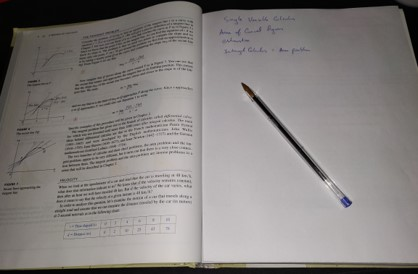
\includegraphics[width=0.5\linewidth]{Figures/book.jpg}
    \caption{A book with a blank sheet of paper slotted between the pages to take notes on}
    \label{fig:enter-label}
\end{figure}

Picture a book with a blank sheet of paper slotted in between each page. As you read, you take notes on this paper and as you flip to the next page, a new sheet awaits you. When it’s time to revise, you go back to that page of the book and the sheet containing your notes on the topic are right there waiting for you.  

No flipping between refill pads, copy-books, documents on your laptop, or in the cloud. No wondering if the notes you took are complete, or if you missed an important point. Everything is in one place. 

Now combine this with digital document management and cataloguing, tagging, searching and linking. It should be trivial to find your notes when you need to refer back. 

This is the feeling note reader wants to achieve. 

Note reader aims to reduce the friction associated with storing and accessing notes and study material. Reduce the cognitive load of note-taking and encourage real-time engagement with the material. 

\section{Contribution}

The application proposed in this project is composed of several key features, such as document reading and rendering, text editing, cataloguing and multiplatform support. To orchestrate these components in a seamless manner, I will leverage the skills and knowledge gained throughout my degree program. 

I will apply user-centred design principles through requirements engineering to ensure NoteReader addresses the clear needs of its intended users. This includes gathering, prioritizing, and validating functional and non-functional requirements.

Adherence to object-oriented design principles (like encapsulation, abstraction, inheritance, and polymorphism) will ensure a cohesive, modular system. Core functionalities like document viewing, note synchronization, and user interaction will be implemented as modular, reusable components.

By following object-oriented design principles, NoteReader will be maintainable and extensible. Changes to one part of the system (like file type support) can be isolated to specific classes or components without affecting the rest of the application. This modular approach ensures scalability as new features are introduced.

NoteReader will be developed using the agile Scrum framework, focusing on iterative development. Emphasis will be placed on early delivery of a minimum viable product (MVP) with successive prototype releases. These iterations will allow for continuous feedback loops and improvement.

Knowledge of agile methodologies will enable me to manage project scope, prioritize features, and ensure timely delivery of new prototypes. Skills in backlog management, sprint planning, and stakeholder collaboration will be demonstrated through well-documented sprints and the inclusion of a feedback process for user testing.

Since NoteReader is a multiplatform solution, user accessibility across devices is a core requirement. The UI must adapt to multiple screen sizes and input methods (desktop, tablet, mobile). By using Kotlin Multiplatform, I will leverage platform-specific adaptations for mobile and desktop environments.

The application will maintain a consistent user experience (UX) across Windows, macOS, Linux, and mobile devices. Designing UI components that work equally well on different devices will showcase the skills I gained from mobile development modules. The ability to seamlessly handle document navigation and note creation across platforms is central to NoteReader's usability.

One of NoteReader's unique value propositions is the use of version control services (like GitHub and GitLab) as a method of synchronizing notes. This method ensures that users have access to their notes across multiple devices while maintaining a revision history of their notes.

This feature demonstrates my ability to develop tools that leverage existing cloud infrastructure to deliver a seamless synchronization experience. My knowledge of Git API integration will allow me to build features for automatic sync, conflict resolution, and file version tracking.

A No-SQL file-system-based approach will be used to store and organize notes, metadata, and links to source documents. This approach provides flexibility in handling diverse data formats (PDFs, Word documents, PowerPoints, etc.) and ensures that all associated notes are easily searchable.

The catalogue file (or index) will be synced alongside the notes themselves in the Git repository. This ensures that the state of the catalogue remains synchronized with user notes, even when accessed from multiple devices.

By using Git for note synchronization, the catalogue must be resilient to merge conflicts and data corruption. The system will be designed to track changes to catalogue files, and where conflicts arise, the system will attempt to resolve them automatically or rebuilding, alerting the user only if manual intervention is required.

\section{Structure of This Document}

This document is organized into the following sections:

\begin{table}[h!]
\centering
\begin{tabular}{|p{5cm}|p{10cm}|}
\hline
\textbf{Section} & \textbf{Description} \\ \hline
Introduction & Outlines the motivation behind the project, the key contributions, and an overview of the document's structure. \\ \hline
Background & Provides context for the project, including its thematic position within computer science, a review of existing solutions, and relevant literature on the topic of digital note-taking and learning efficiency. \\ \hline
Problem Definition & Discusses the core challenges that the project seeks to address, outlining existing issues with current solutions and presenting the objectives and functional requirements of the proposed application. \\ \hline
Implementation Approach & Details the methodology used to develop the application, including user flows, architectural design, technologies, risk assessment, and the implementation timeline. \\ \hline
Implementation & Details the actual implementation of the project and difficulties encountered. \\ \hline
Testing and Evaluation & Breaks down the methods used to evaluate progress \\ \hline
Conclusions and Future Work & Summarizes the findings and learnings of the project, reflects on the challenges encountered, and outlines potential future developments. \\ \hline
Appendices & Includes supplementary materials such as code snippets, wireframe models, and diagrams to support the main text. \\ \hline
\end{tabular}
\caption{Structure of This Document}
\label{tab:document_structure}
\end{table}


 % Introduction
\chapter{Background}
\label{chap:background}
\lhead{\emph{Background}}

\section{Thematic Area within Computer Science}

The project of developing NoteReader, lies at the intersection of educational technology (EdTech) and software development. EdTech is a rapidly evolving field characterized by the integration of modern technologies into learning environments to enhance educational outcomes. Current trends in EdTech include the use of AI-driven personalized learning systems, immersive experiences through AR/VR, and data-driven analytics for adaptive learning paths.

However, unlike many modern EdTech initiatives that prioritize AI or AR/VR enhancements, this project addresses a more fundamental aspect of learning, the effective organization and access of study materials. By tackling the challenge of document-linked note-taking, NoteReader aims to simplify the learning process, reduce cognitive load, and enable efficient study workflows. Foundational learning strategies are essential, even as new technologies emerge.

To achieve its goals, this project draws upon principles from several key areas of computer science. These areas provide the theoretical and practical foundations required to develop a robust, scalable, and user-friendly application.

\section*{ACM Computing Classification System (CCS) Concepts}

\noindent
\textbf{Human-centered computing:} User interface design\\
\textbf{Information systems:} Document collection models\\
\textbf{Information systems:} Search interfaces\\
\textbf{Software and its engineering:} Software creation and management


 \section{A Review of Currently Available Alternatives}
This section reviews existing note-taking and document reading solutions to identify gaps in the market that NoteReader aims to fill. Key gaps include the lack of seamless integration between document viewing and note-taking, insufficient support for a wide range of document formats, limited cross-platform compatibility, and reliance on costly subscription-based cloud syncing services. 

Addressing these issues, NoteReader aims to provide a unified, subscription-free, and cross-platform solution that enables document-linked notes, multi-format support, and intuitive cataloging and search capabilities. The insights provided here will support the rationale for developing NoteReader and highlight the need for an integrated solution.

\subsection{Existing Note Taking Solutions}
    The findings below are based on my research into the feature availability of several note taking applications. This information is documented in an excel sheet. See attached file Existing Solutions Spreadsheet: \attachfile{existing_solutions.xlsx}. 
    
    A small excerpt of this file can be found in figure~\ref{fig:CD}.

    \begin{figure}
    \centering
    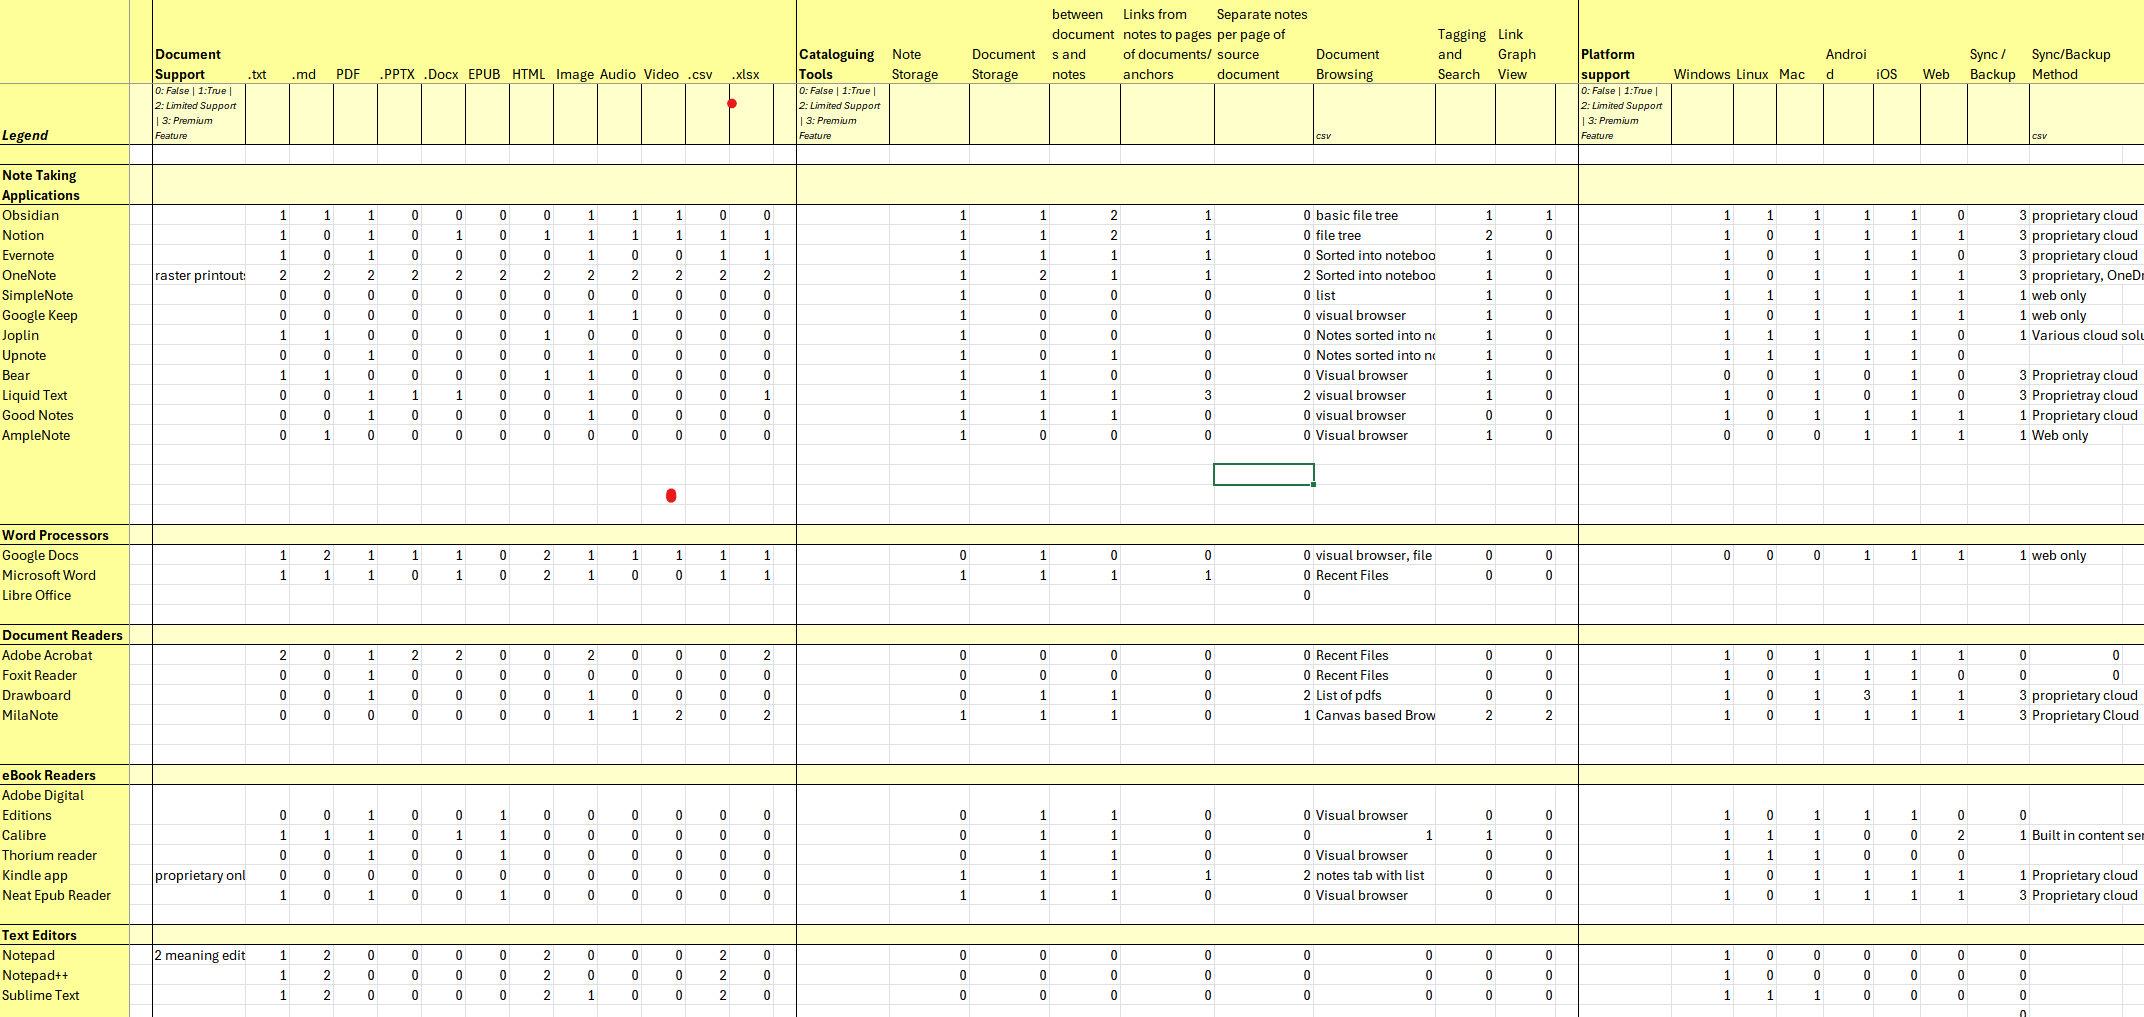
\includegraphics[width=1\linewidth]{Figures/existing solutions excerpt.png}
    \caption{Excerpt from the Existing Solutions Excel File, displaying some key findings (including document file-type support, cataloguing options and platform support)}
    \label{fig:Existing}
    \end{figure}

    \begin{figure}
        \centering
        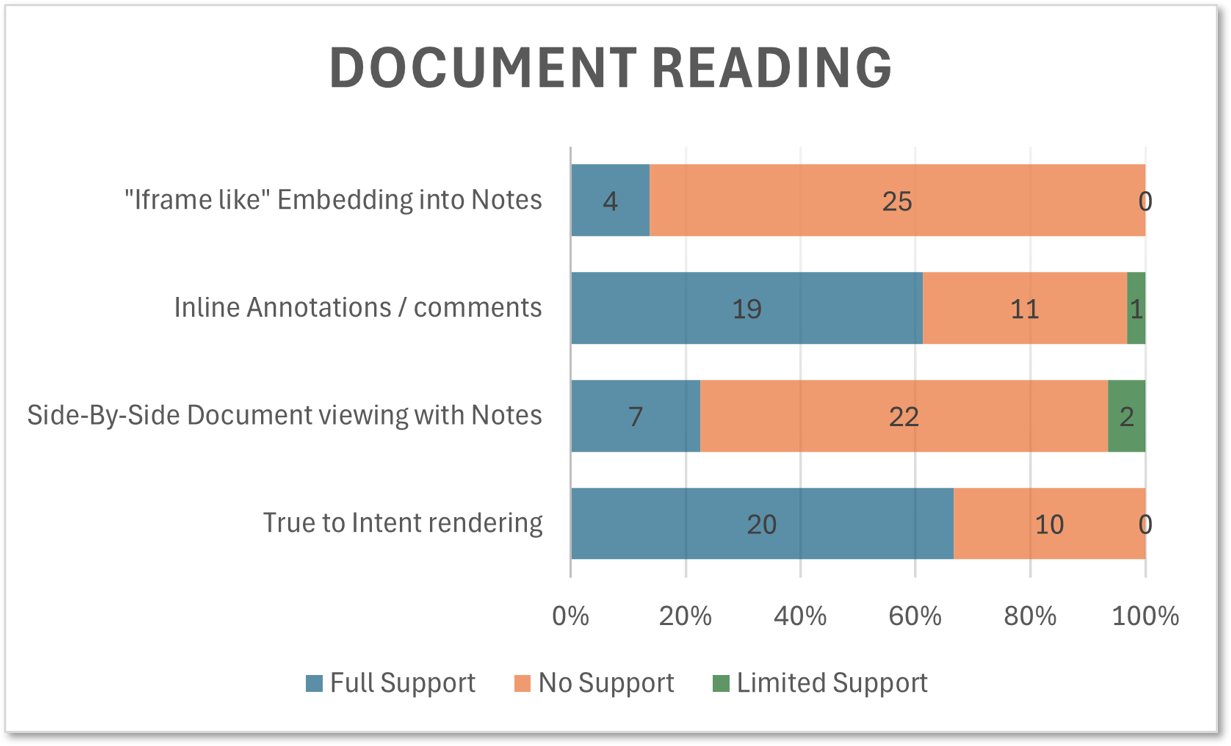
\includegraphics[width=1\linewidth]{Figures/docreading.png}
        \caption{Graph illustrating the support across reviewed applications for features including "True to Intent Rendering" and "Side by Side Viewing"}
        \label{fig:enter-label}
    \end{figure}
    \begin{figure}
        \centering
        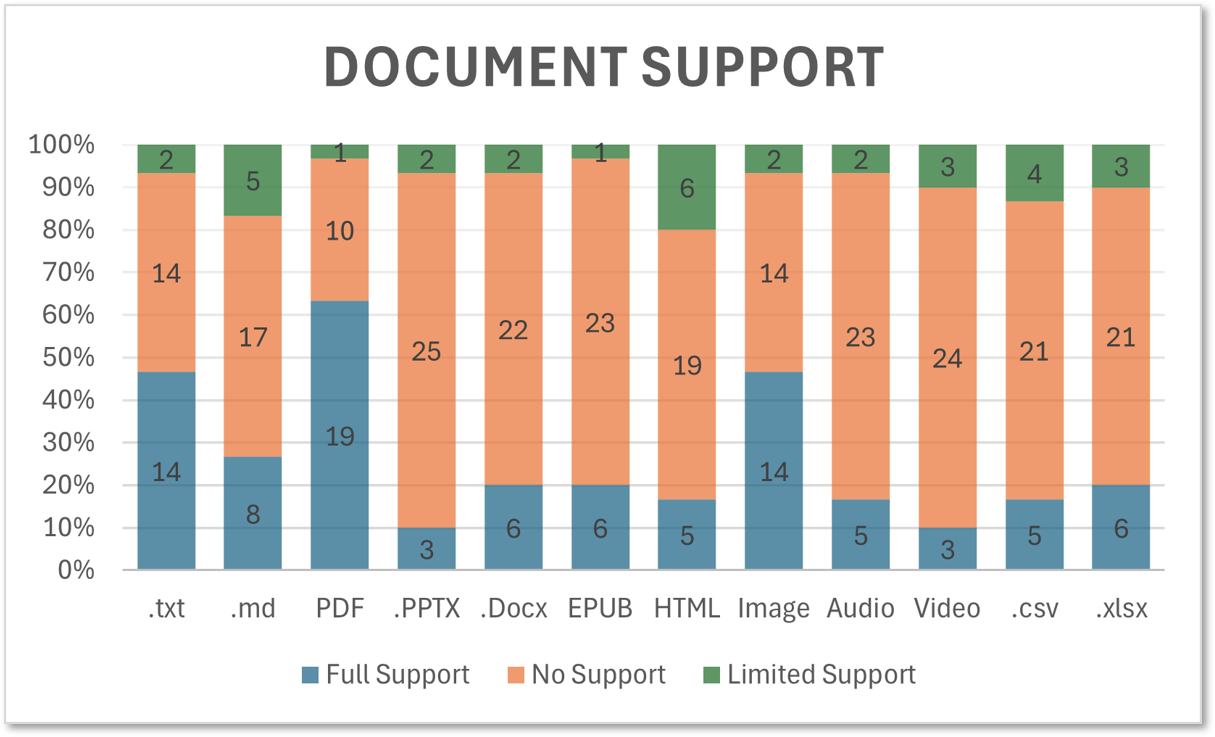
\includegraphics[width=1\linewidth]{Figures/docsupp.png}
        \caption{Graph illustrating the support across reviewed applications for document format}
        \label{fig:enter-label}
    \end{figure}
    \begin{figure}
        \centering
        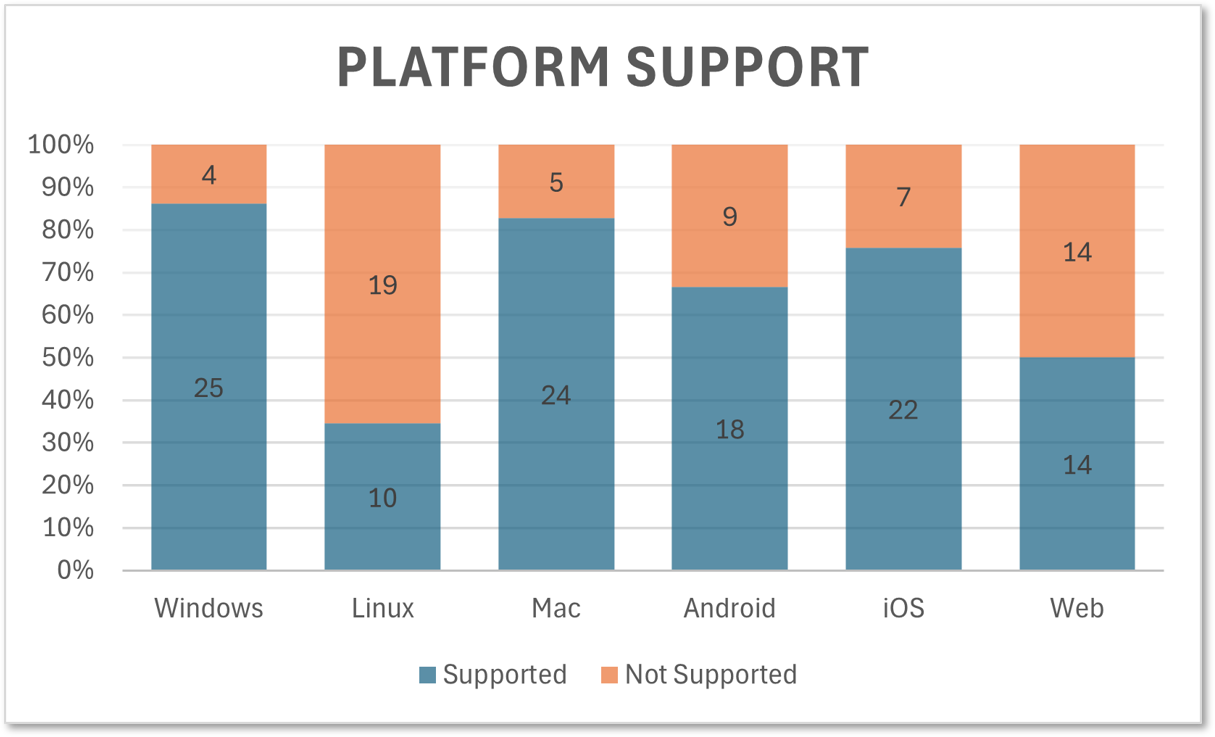
\includegraphics[width=1\linewidth]{Figures/platsupp.png}
        \caption{Graph illustrating the support across review applications for different platforms}
        \label{fig:enter-label}
    \end{figure}
    
	\begin{enumerate}
	    \item \textbf{Document file type support.} \\
        Very few applications support a wide range of common document types, and those which do do so using destructive methods, like raster printing of the document to a canvas, without storing the original. 
        
	    \item \textbf{File Syncing} \\
        Most note taking applications require a proprietary cloud service to sync between devices, or back up files. \\
        Version Control with remote repositories are not commonly used as a method of syncing this data.
    
	    \item \textbf{Dual functionality } \\
        Most document readers only allow notes via annotations, while most note taking applications only support document reading as embedded files. \\ 
        The ability to have side by side note taking and document reading is uncommon.
        
	    \item \textbf{Page of Notes per Page of Document} \\
        No application fully supports having linked notes with a separate page of notes per page of source document. Those which do support a similar function do so by adding all notes and pages to a large canvas for example Microsoft One Note. 
        
	    \item \textbf{Platform support.} \\
        Most applications tend to support only a couple of platforms. Linux support is especially rare for multiplatform applications.  
        
	    \item \textbf{Cost} \\
        Most note taking applications require some form of monthly subscription to use to their full potential. The pricing varies widely, as do the features on offer.
        
	\end{enumerate}

 \section{A Review of literature available on the effectiveness of digital note taking}

    In this section, I will review available literature on studies performed on the effectiveness of digital note taking, when compared to handwritten notes. 
    
    This review aims to better understand the benefits of the digital note-taking process to inform the development of NoteReader's user experience. The literature provides insight into the cognitive, procedural, and organizational aspects of digital note-taking, helping shape the design of the tool to meet the needs of learners.
 
    
    \subsection{Note-taking and Handouts in The Digital Age\cite{stacy_note_taking_2015}}

    In this article, the author explores the role of Handouts in lectures as a supplemental tool. The author discusses a number of challenges regarding handouts, pointing out that detailed handouts may lead to students not engaging in lectures, and simply memorizing the power point slides. They also suggest that a complete lack of handouts may result in students transcribing the full lecture material, rather than engaging in real time. 

    A compromise is suggested, where "skeletal" notes will provide a "scaffolding". This method gives a structure to note taking, without providing all information in the handouts themselves. The conclusion the author reaches here is that the student would be required to engage with the material, but not need to fully transcribe, just fill in the gaps. 

    This philosophy aligns well with the intended purpose and functionality of NoteReader. Source material acting as a scaffolding for personal notes, would be well supported by an application where pages of notes are displayed alongside pages of source material.

    By offering a side-by-side view, NoteReader facilitates a structure where students can engage deeply with the material without the cognitive overload of transcription.
    
    \subsection{Effectiveness of Digital Note-Taking on Students’ Performance in Declarative, Procedural and Conditional Knowledge Learning\cite{Sun2019}}
    
    This article describes a small trial of 72 Students, 40 taking digital notes, and 32 taking conventional handwritten notes. The author refers to three forms of knowledge Declarative, Procedural and Conditional, to differentiate between understanding of factual information, understanding of processes, and understanding of when to apply knowledge. Each will be measured separately in their study, and based on performance students are divided into percentiles. Notably this study focused on Computer Science students, in programming only. 

    Excellent students (those in the 70th percentile) showed improvement in all three knowledge types, but especially in declarative knowledge when using digital notes. Students below the 30th Percentile showed significant improvement in Conditional knowledge. Mid level students did not show significant improvement. 

    No group showed a decrease in performance when using digital notes. While this is a relatively small study, there is a suggestion that the advantages of digital note taking may be at least as effective as traditional methods. 

    The additional features proposed by NoteReader may be beneficial in further improving the performance difference of students taking digital notes. The split view link between source material and notes will allow students to study with improved context which may improve conditional understanding, when compared to memorization. This structured support mirrors the scaffolding identified as effective in the previous study\cite{stacy_note_taking_2015}.

    \subsection{Taking notes in the digital age: Evidence from classroom random control trials\cite{Artz2020}}
    
    This article describes a study to compare the effectiveness of digital note-taking compared to handwritten notes. 

    Some key findings were that exam scores showed no statistically significant difference between digital and handwritten notes. 
    
    There was however evidence that in subjects with high dependence on graphical or mathematical elements digital note taking may be at a disadvantage. Digital methods of creating diagrams, or mathematical equations tend to be more difficult and slower. 

    While not in scope for the initial round of development of NoteReader, inclusion of handwriting support and OCR may be a valuable addition to compensate for these weaknesses in a future release.  % Background
\chapter{Problem - \thesistitle}
\label{chap:problem}
\lhead{\emph{Problem Statement}}
% The key question to be addressed in this chapter is: "What do I want to achieve".

% This chapter should comprise around 1500 words and describe the problem you are trying to solve. Try to be as specific here as you can, this will help you to anticipate possible risks such as lack of support from APIs.

\section{Problem Definition}
% Describe the problem you are trying to solve in this project. 

In the modern era of digital learning, the process of note-taking has undergone a fundamental shift from traditional paper-based methods to digital mediums. Despite the availability of numerous note-taking applications and document readers, there exists a significant gap in the seamless integration of these two functionalities. Most current solutions treat either note-taking or document reading as the primary focus, with the other as an ancillary feature. This approach introduces friction into the study process, as users are forced to toggle between multiple applications to take notes and reference study materials.

The proposed solution, NoteReader, aims to address this problem by creating an all-in-one, platform-agnostic application that treats both document reading and note-taking as first-class priorities. The primary objective is to develop a cohesive system that allows users to read and annotate documents, create linked notes, and access these materials in an organized and intuitive manner.


\subsection{Current Issues}

\begin{itemize}
    \item Fragmentation of Tools: Current market solutions (e.g., Microsoft OneNote, Adobe Acrobat) often excel in one area while providing minimal support for the other. Users are forced to switch between dedicated document readers and standalone note-taking applications, leading to a disjointed study experience.
    \item Limited Multi-Platform Support: Existing applications frequently prioritize Windows, macOS, or mobile platforms, but fail to offer full support across all devices, especially Linux.
    \item High Cost of Subscription Services: Many applications rely on proprietary cloud storage systems (e.g., Evernote, Notion) to sync notes, necessitating paid subscriptions for cross-device access. This raises the financial barrier for students and educators.
    \item Inadequate File Type Support: Current solutions support only a limited number of document formats. For example, EPUBs and PowerPoint slides are often not supported natively or require costly add-ons.
    \item Loss of Context: Existing applications do not associate notes with the specific page or section of the source material they reference, making it difficult for users to revisit contextual notes.
    \item Manual Organization and Storage Issues: Users are required to manually organize notes and study materials, often leading to misplaced documents and incomplete notes.
    \item Data Portability: Many note-taking applications lock users into proprietary formats that limit the ability to transfer or back up notes independently. This can be a critical issue if users decide to migrate to another platform.
\end{itemize}

\subsection{Proposed Solutions}
NoteReader proposes a unified application that simultaneously handles document reading and note-taking, offering a "split-view" interface where documents are displayed alongside a corresponding note pane. This side-by-side approach ensures that users can create notes that are contextually linked to specific pages or sections of the source document.

\begin{itemize}
    \item Split-View Interface: Each document opened in NoteReader creates a linked folder containing all notes relevant to that document. As users navigate through the document, the corresponding notes automatically load, ensuring users maintain contextual continuity.
    \item Multi-Platform Compatibility: Built using Kotlin Multiplatform, NoteReader will be available on Windows, macOS, Linux, and mobile devices, providing true cross-platform accessibility.
    \item Offline and Cloud-Backed Storage: Notes and documents are stored locally in plain text, ensuring data portability. Optional synchronization with GitHub or other version control platforms provides cloud-based backup and version history.
    \item File Format Versatility: Support for a wide array of document formats, including PDF, DOCX, EPUB, PPTX, TXT, CSV, and more. This eliminates the need for users to convert files to compatible formats.
    \item Contextual Note-Linking: Notes are linked directly to specific pages of the source document, allowing users to jump directly to the source context with a single click.
    \item Lightweight, Portable Note Files: All notes are saved as plain text files, making them accessible and editable with other tools like Obsidian or any plain text editor.
    \item Tagging, Searching, and Categorization: Users can categorize and tag notes for quick access, supporting efficient search and retrieval of information.
    \item Version Control for Notes: Sync and track changes to notes using Git-based version control, offering a history of note revisions and easy restoration of previous versions.
\end{itemize}

\section{Objectives}
% Enumerate the objectives you want to achieve in your project. Again as this is an early stage these will tend to change but there should be a rational explanation for this change. Always document your work, keep a lab book during the term that you only use for FYP!
\subsection{Scope}
\begin{itemize}
    \item Create a Seamless Note to Document Link: Achieved through file system,  Ensure users can link notes to specific document pages, making it easy to reference the original context.
    \item Achieve Multi-Platform Support: Use Kotlin Multiplatform, or similar frameworks, to provide cross-platform compatibility across Windows, macOS, Linux, and mobile devices
    \item Facilitate Data Portability: Ensure that users' notes are stored in plain text files and that the application supports exporting notes for use in other tools like Obsidian to prevent vendor lock in. 
    \item Optimize UI/UX for Cognitive Load: Design an intuitive user interface that reduces cognitive load during note-taking, focusing on minimalist design and efficient navigation.
    \item Offer Customization and Personalization: Allow users to tag, categorize, and search notes, providing tailored organization options for diverse user needs.
    \item Minimize Cost and Friction: Avoid reliance on proprietary cloud services or subscription fees by using open formats, local storage, and optional Git based version control and sync.
\end{itemize}

\subsection{Stretch-Goals}
The following is a list of features which I would consider to be important for a final version of this project, but are not necessarily core to the functionality of a Minimum Viable Product or Prototype release. 

These will be explored, time allowing, after the core scope is implemented. 

\begin{itemize}
    \item OCR for Images: Implement Optical Character Recognition (OCR) technology to convert scanned images and PDF documents into searchable and editable text. This functionality will enhance accessibility and improve the discoverability of text-based content in image files.
    \item Handwriting Support: Enable handwriting support for touchscreen devices and styluses, allowing users to write notes directly on the document. This approach will appeal to users who prefer handwritten notes and facilitate better physio-cognitive engagement with the study material.
    \item Dictation: Introduce voice-to-text dictation features, allowing users to transcribe spoken words directly into notes. This will benefit users who prefer to dictate notes during lectures or meetings, enabling fast, hands-free note creation.
    \item Video and Audio, Lecture Recording with Timestamps: Develop functionality for recording live lectures or video content. Users can take time-stamped notes that are linked to specific moments in the video / sound clip, allowing them to quickly revisit relevant sections during playback.
\end{itemize}

\subsection{Out of Scope}
The following are a list of potentially valuable additions, which fall outside the core purpose of the application. These may be useful features to provide in future updates, but will not be the focus of this project. 

\begin{itemize}
    \item AI Integration: The initial version of NoteReader will not include AI-driven features such as natural language processing (NLP), automated content summarization, or predictive note suggestions.
    \item Web Interface: The NoteReader application will be a desktop and mobile application only, with no support for web browsers or cloud-based interfaces.
    \item Real-Time Collaboration: Multi-user editing or real-time collaborative note-taking is outside the scope of the initial implementation.
    \item Cloud-Only Storage: While cloud sync via GitHub is supported, the system will not offer a proprietary, always-online cloud storage solution.
\end{itemize}

\subsection{Stakeholders}
\begin{itemize}
    \item Students: Students across various academic disciplines are the primary beneficiaries, as NoteReader facilitates efficient study workflows and better information retention.
    \item Researchers and Academics: Researchers who must organize large collections of study materials and notes for literature reviews and projects will benefit from the system’s tagging, linking, and search capabilities.
    \item Educators and Lecturers: Educators can create lecture notes and materials linked to specific document pages, offering students an interactive and guided learning experience.
    \item Journalists: Journalists who need to organize interview notes, source materials, and articles can use NoteReader’s organizational capabilities.
\end{itemize}



\section{Functional Requirements}
% Enumerate the functional requirements you want your project to have. 

% Please, do not include the use cases here. If you want to create a one-to-one mapping between functional requirements and use cases (which does not necessarily need to be the case, indeed most likely this will not be the case) do it elsewhere. Here should purely describe what do you want to do. In no case should you use this section to provide a description of how to implement them, that is for later. For people doing projects that are not heavy implementation projects (e.g. deploying an architecture or testing a novel tool in specific conditions) this structure can still be used as it will force you to think about what you plan to achieve and what possible metrics you may need to measure success.

% Let me explain this with more detail. A common mistake is that people confuse the problem description with the solution approach. This is a common mistake by confusing the \emph{what} with the \emph{how}. Here we are purely focused on the what: What is this project about? What are the objectives? What are the functional and non-functional requirements? 

% How are we going to do all these things? Well, this is a question for next chapter. Provided a problem, an objective or a functional requirement, obviously there will usually be many ways of doing it, thus there will be many \emph{hows}, but the definition, the \emph{what} we want to achieve will be unique.

% One other display structure you may wish to use at some stage during the report is a figure array. This can also be easily done with Latex and is shown in figure \ref{fig:twosuccesskid}

% \begin{figure}
% \centering     %%% not \center
% \subfigure[Figure A]{\label{fig:a}
\includegraphics[width=0.48\textwidth]{successkid.jpg}}
% \subfigure[Figure B]{\label{fig:b}
\includegraphics[width=0.48\textwidth]{successkid.jpg}}
% \caption{Two Success kids}
% \label{fig:twosuccesskid}
% \end{figure}

\begin{itemize}
    \item The system shall provide a split-view interface to allow users to view documents and take notes simultaneously.
    \item The system shall support the import and display of PDF, EPUB, DOCX, and PPTX files
    \item The system shall allow users to link notes to specific pages or sections of the source document.
    \item The system shall support searching and filtering of notes and documents using tags, keywords, and categories.
    \item The system shall support exporting notes in plain text format for use in other applications.
    \item The system shall enable users to sync notes to cloud storage providers like GitHub using version control.
    \item The system shall allow users to tag and categorize notes for efficient organization and retrieval.
\end{itemize}

\section{Non-Functional Requirements}
\begin{itemize}
    \item Performance: The system shall load and display documents without noticeable wait times on standard modern devices.

    \item Usability: The user interface shall be intuitive, with clear user experience flows. 

    \item Scalability: The system shall support large document files (over 25mb), and offer alternative synchronization methods for these files. 

    \item Portability: The system shall support cross-platform functionality on Windows, macOS, Linux, and mobile devices.

    \item Reliability: The system shall gracefully handle unexpected crashes to prevent data loss by saving notes in real-time and automatically restoring the last working state upon restart.

    \item Maintainability: The system shall be modular to allow for easy updates and addition of new features.

    \item Compatibility: The system shall be compatible with widely used file formats (PDF, EPUB, DOCX, PPTX, TXT, etc.).
\end{itemize}


 % Problem Analysis and Design
\chapter{Implementation Approach}
\label{chap:implementation}
\lhead{\emph{Implementation Approach}}

\section{User Flow} 
In order to create a well-designed, purposeful user interface (UI) for the NoteReader application, it is essential to understand and model how users interact with the system. To achieve this, I have created a series of user flow diagrams that represent key workflows within the application. These diagrams illustrate the sequential steps users take to complete specific tasks, ensuring that the interface is intuitive and aligns with user expectations.

The following user flows have been designed:

\begin{itemize}
    \item \textbf{Document Import, Reading, and Note Taking Flow} (see Figure~\ref{fig:Document Import, Reading and Note taking Flow}): 
    This flow captures the process a user follows to import a new document into the application, read the document, and take notes alongside it. It begins with the user selecting a document from their file system, proceeds through the rendering of the document in the split-view interface, and describes how notes are created, saved and reloaded. 

    \item \textbf{Opening Already Imported Documents from Catalogue Flow} (see Figure~\ref{fig:OpeningAlreadyImportedDocuments}): 
    This flow models the steps for accessing previously imported documents via the application's catalogue or library. Users can search for, sort, and select documents from their collection. Once selected, the application loads the document alongside the corresponding notes for the user to resume their work seamlessly.

    \item \textbf{Git-Based File Synchronization Flow} (see Figure~\ref{fig:gitBasedSync}): 
    This flow explains how the application handles file synchronization using a Git-based version control system. It includes steps for committing local changes, pulling updates and pushing notes and metadata to a remote repository to ensure consistency across multiple devices. Conflict resolution and large file size (LFS) are also considered in this flow to provide a smooth syncing experience.
\end{itemize}

\subsection{Document Import, Reading, and Note Taking Flow}
This user flow begins when the user selects a document for import. The application processes the document, creating a folder in the user's file system to store notes linked to the document. The document is displayed in the split-view interface, with the left pane dedicated to rendering the document and the right pane for note-taking. The user can navigate through the document, take notes, and save them automatically. Notes are stored in lightweight plain-text files for portability.

\subsection{Opening Already Imported Documents from Catalogue Flow}
In this workflow, the user starts by accessing the application's catalogue or library. They can search for a document using keywords, tags, or filters. Once the desired document is located, the application loads it into the split-view interface, along with previously saved notes. This ensures that the user can seamlessly continue their work without losing context.

\subsection{Git-Based File Synchronization Flow}
The synchronization flow focuses on maintaining consistency across multiple devices. Users can commit their local changes (e.g., notes, updates to the catalogue) and push them to a remote Git repository. If working on another device, they can pull updates from the remote repository to retrieve the latest notes and document metadata. The system handles merge conflicts by alerting users and providing options for manual or automatic conflict resolution.

These user flows ensure that NoteReader is user-centric, intuitive, and aligned with the expectations of students, researchers, and other users. Detailed diagrams for each flow are provided in Figures~\ref{fig:DocumentImportFlow}, \ref{fig:OpeningAlreadyImportedDocuments}, and \ref{fig:GitBasedSync}, respectively.


\section{Architecture} \label{sec:Arch}
% Describe the architecture of the solution that you have in mind, including:
% \begin{itemize}
%     \item Technologies involved (e.g., frameworks, programming language). 
%     \item The hardware needed to develop the project (and to support at deployment stage)
% \end{itemize}

% Provide a high level view of the system you have in mind, including any package of classes, what is it responsible for and what other packages it communicates to. Provide a high level view of the database (or structure) needed to support the project, including what each table/document is responsible for and the hierarchy among them. You need to be as specific here as you can, why? Because this will aid you in identifying parts of the project you are vague on, this may be fine for some components but cause problems in term 2 for others. If you have hardware element in your project this is also where you provide a high level view of how these elements integrate into the project. So for a project that is cyber-physical you will have both a hardware and software architectural diagram. N.B. This is NOT a full system design but a high level overview of what you can credibly develop. This architecture should be informed by prototyping activity. 

% Some of the implementation focused projects may describe how do you envision tackling the functional requirements of your project via a set of use-cases. DFDs are also helpful here to understand elements of your project that may cause problems. You should describe the role of the different parts of the architecture of the solution, and the interaction among them.

\subsection{Technologies}
\begin{itemize}
    \item Kotlin Multiplatform: Chosen for its ability to support multiple platforms, including Windows, macOS, Linux, and mobile devices.
    Below is a brief review of a number of other multiplatform frameworks that were considered.
        \begin{itemize}
            \item \textbf{Maui:}\\
            A multiplatform framework which is part of the .NET ecosystem. This framework supports multiple operating systems, but notably lacks Linux support.
            
            \item \textbf{React Native:} \\
            \href{https://reactnative.dev/docs/out-of-tree-platforms}{React Native Platform Support}\\
            Supports all common platforms, though Linux support is community driven
            
            \item \textbf{Electron:}\\
            Chromium based, supports all desktop platforms, but does not support mobile
            
            \item \textbf{Flutter:} \\
            \href{[https://docs.flutter.dev/reference/supported-platforms}{Supported Platforms}\\
            Broad support in Java Script based framework by google
            
        \end{itemize}

    \item Document Frameworks: 
    These frameworks are potential solutions for handling document parsing and rendering. The actual solution may change over the course of development. 
    
        \begin{itemize}
            \item Markdown/HTML Support: Used to format notes and support plain-text storage, ensuring compatibility with other note-taking applications like Obsidian.
            
            \item \textbf{.pdf:} \\
            The PDF format is well defined, under ISO standard 320000-1. \\
            PDF.js would be one option, for displaying this document type, through a platform independent web view. 
            
            \item LibreOffice: Used to convert PowerPoint and Word files to PDF for consistent rendering.
            
            \item \textbf{Images (.png, .jpeg, .webp, etc)}\\
            These can easily be displayed either directly in app, or using a web view. 
            
            \item SheetJS: Used to render CSV and XLSX files.
            
            \item Used for rendering eBooks in EPUB format.
            
        \end{itemize}

        Regardless of the specific framework used, the architecture of the solution remains the same. An interface will be defined for document rendering, with each document type being defined as an implementation of that interface. 
    
        This ensures the functionality is standardized, and provides a clear pathway for adding additional document format support in future releases. 

    \item Integrations with existing Systems
    \begin{itemize}
        \item Git, with GitHub/GitLab: Integration with version control for note synchronization.
        \item OCR (Optical Character Recognition): Tesseract is proposed for text recognition in image-based PDFs.
        \item Handwriting Recognition: Windows Ink support for annotating notes on touch-enabled devices.
    \end{itemize}
\end{itemize}


\section{Risk Assessment}
% Identify any potential risk precluding you from successfully complete your project. This section is really important and often neglected by students resulting in fatal risks occurring in some projects. Make sure to give this section the time it requires. Classify the risk according to their importance, possibility of arising and enumerate the decisions you can make to anticipate them or mitigate them (in case they finally arise). Table \ref{tab:ProjRisks} may help with this classification. This section should include your mitigation approach for any critical risks.

\begin{table}[h]
\centering
\scriptsize
\caption{Initial risk matrix}
\begin{tabular}{|p{2cm}|p{2cm}|p{2cm}| p{2cm} |p{2cm}| p{2cm}|}
\hline \bf Frequency/ Consequence & \bf 1-Rare & \bf 2-Remote & \bf 3-Occasional & \bf 4-Probable & \bf 5-Frequent\\ [10pt]

\hline \bf 4-Fatal & \cellcolor{yellow!50} & \cellcolor{red!50} & \cellcolor{red!50} & \cellcolor{red!50} &\cellcolor{red!50} \\ [10pt]

\hline \bf 3-Critical &\cellcolor{green!50} & \cellcolor{yellow!50} & \cellcolor{yellow!50} & \cellcolor{red!50} &\cellcolor{red!50} \\ [10pt]

\hline \bf 2-Major & \cellcolor{green!50} & \cellcolor{green!50} & \cellcolor{yellow!50} &\cellcolor{yellow!50} &\cellcolor{red!50} \\ [10pt]

\hline \bf 1-Minor & \cellcolor{green!50} & \cellcolor{green!50} & \cellcolor{green!50} &\cellcolor{yellow!50} &\cellcolor{yellow!50} \\ [10pt]
\hline
\end{tabular} \\
\label{tab:ProjRisks}
\end{table}

\begin{table}[h]
\centering
\caption{Risk Table for Identified Risks}
\begin{tabular}{|l|c|c|}
\hline
\textbf{Risk}                           & \textbf{Frequency} & \textbf{Consequence} \\
\hline
\rowcolor{yellow!50} Scope Creep        & Occasional        & Major                 \\
\hline
\rowcolor{red!50} File Corruption       & Remote            & Fatal                 \\
\hline
\rowcolor{yellow!50} Merge Conflicts    & Frequent          & Minor               \\
\hline
\rowcolor{green!50} Large File Sizes   & Rare              & Major                 \\
\hline
\end{tabular}
\label{tab:ProjRisks}
\end{table}

\subsection{Risk Identification}
\begin{itemize}
    \item Scope Creep: The addition of features like OCR or audio-visual notes early on could divert development focus.
    \item File Corruption: Data loss could occur due to file corruption during version control sync.
    \item Merge Conflicts: Users may encounter conflicts when syncing files via Git.
    \item Large File Sizes: Some file types (e.g., PowerPoint) may be too large for GitHub’s file size limitations.
    \item Change in GitHub terms: A change in the terms of service for remote version control repositories may impact the functionality of the application. 
\end{itemize}

\subsection{Risk Mitigation Strategies}
\begin{itemize}
    \item Agile Methodology: Use Scrum with two-week sprints to maintain a clear development timeline.
    \item Data Backup: Ensure automatic backups for critical files during sync.
    \item File Locking: Implement a file-locking mechanism during note editing to prevent conflicts.
    \item File Size Limitations: Break large files into smaller components if necessary, or consider cloud storage as a fallback option.
    \item Support multiple git remote services. 
\end{itemize}


\section{Methodology}
% Describe your personal approach on how to tackle the different parts of this project, including:
% \begin{itemize}
%     \item How to tackle the needed research to fulfill the background chapter. 
%     \item How to set up your Computer Science skills to the project needs (e.g., describe your plan to learn any new technology involved on the project that you are not familiar with). 
%     \item What core project managing approach will you follow (e.g., Waterfall, Scrum, etc).
% \end{itemize}



\section{Implementation Plan Schedule}
Agile Scrum: Six sprints of approximately two weeks each will be used to track development progress. These Sprints will start alongside semester 2. 

Technology Familiarization: Time between now and the beginning of Sprint 1 will be allocated to learning Kotlin Multiplatform and Git API integration.

\begin{itemize}
    \item Sprint 1: PDF and Text Editor with Linked Pages.
    \item Sprint 2: Document and Note Cataloguing and Search.
    \item Sprint 3: Improved Document Format Support.
    \item Sprint 4: Version Control and Sync.
    \item Sprint 5: UI/UX Enhancements.
    \item Sprint 6: Prototyping and Integration of Additional Features.
   
\end{itemize}

The schedule allows for iterative feedback and testing, ensuring that each module is stable before moving forward.

\section{Evaluation}
\subsection{Functional Testing}
\begin{itemize}
    \item Document Rendering: Ensure support for PDF, DOCX, EPUB, and PPTX files.
    \item Note Sync: Test sync functionality across GitHub and other remote services.
    \item Tagging and Search: Verify that tagging and search features are intuitive and fast.
\end{itemize}

\subsection{Non-Functional Testing}
\begin{itemize}
    \item Performance: Measure document load times and ensure responsiveness for large files.
    \item Portability: Ensure the system works across Windows, macOS, Linux, and mobile platforms.
    \item Reliability: Test for system stability during crashes and validate automatic recovery.
\end{itemize}
% Come up with an evaluation plan that allows you to measure how much have you actually achieved the goals of your project. This again is a section that is often neglected where students loose marks. How do you plan to measure the output of your project? A binary it works/does not work is insufficient. You need to be able to quantify the success against both the functional requirements and the initial idea. These are not the same as you may meet all function requirements outlined but not solve the overall problem because you have failed to revisit these and update them with new information which you learn as you are developing the project.

\section{Prototype}
Each sprint will deliver an executable iteration of the project. 

A prototype will be developed by the end of Sprint 4. This prototype will feature all core functionality:
\begin{itemize}
    \item Document Viewing: View and navigate PDF, DOCX, EPUB, and PPTX files.
    \item Note Editor: Create and store notes linked to specific pages.
    \item Version Control: Sync notes using GitHub.
    \item Split-View: User interface supporting simultaneous document view and note-taking.
\end{itemize}

The prototype will be a minimally viable product (MVP) that focuses on essential functionality, with stretch goals like OCR and handwriting support introduced in later sprints.

For visual reference, several mock ups and diagrams have been produced (See Appendix B.).

\begin{itemize}
    \item A UML Class diagram detailing the high level architecture is displayed in figure~\ref{fig:CD}.
    \item A sample UI for the PC version is represented in figure~\ref{fig:NoteReaderMock}.
    \item A sample UI for the Mobile version of the application is represented in figure~\ref{fig:NoteReaderMobileMock}
\end{itemize}






% Although you do not have a fully functional project yet, you should show wireframes, snapshots or representation on how do you envision your project to look once the implementation phase has been completed. The nature of this section will vary significantly from project to project and can include anything from code snippets to snapshots of service deployments. Any prototyping you have done during the term should be summarized here that has not been captured in earlier sections. For example if you are planning to host your project using AWS in an EC2 instance you should have at least created a "hello world" setup to determine the basics, this probably should have been discussed in section \ref{sec:Arch}. % Implementation Approach
\ifnum \value{semester}=1
\chapter{Conclusions and Future Work}
\label{chap:conclusions}
\lhead{\emph{Conclusions}}

\section{Discussion}
This research phase of the NoteReader project has been instrumental in identifying and understanding the critical challenges and opportunities in integrating document reading and note-taking. The work focused on analyzing existing solutions, exploring technical frameworks, and conceptualizing a solution that addresses the gaps in current tools.

\subsection{Key Considerations}
\begin{itemize}
    \item \textbf{Fragmented Existing Solutions:} Existing tools often focus on either document reading or note-taking, creating a gap in unified functionality.
    \item \textbf{Technical Feasibility:} Ensuring multiplatform compatibility, especially with varying operating systems, was identified as a core challenge for future implementation.
    \item \textbf{User Experience Design:} Balancing functionality with simplicity highlighted the need for iterative user feedback to ensure an intuitive interface.
    \item \textbf{Data Synchronization Concerns:} Utilizing version control systems like Git
\end{itemize}



\section{Conclusion}
The research conducted during this phase underlines the need for a unified application that seamlessly integrates document reading and note-taking. The primary insights include:

\begin{enumerate}
    \item \textbf{Clear Market Gap:} There is a significant gap in the market for tools that prioritize both document reading and note-taking equally.
    \item \textbf{Technological Opportunities:} Technologies like Kotlin Multiplatform and Markdown support offer viable paths to create a flexible and scalable application.
\end{enumerate}

\section{Future Work}
The next steps involve transitioning from the research phase to implementation, focusing on the following areas:

\subsection{Prototype Development}
\begin{itemize}
    \item Build a functional prototype focusing on core features such as document rendering and contextual note-taking.
    \item Test the prototype for usability and cross-platform functionality.
\end{itemize}

\subsection{Technical Enhancements}
\begin{itemize}
    \item Explore and integrate frameworks like PDF.js and Tesseract for document rendering and OCR capabilities.
\end{itemize}

\subsection{User Feedback}
\begin{itemize}
    \item Conduct user surveys and usability tests to gather insights on interface design and feature prioritization.
    \item Refine the design based on iterative feedback.
\end{itemize}

\subsection{Advanced Features (Stretch Goals)}
\begin{itemize}
    \item Investigate the feasibility of integrating handwriting recognition and voice-to-text dictation.
\end{itemize}

 % Semester 1 conclusion
\else
\chapter{Implementation}
\label{chap:imp}
\lhead{\emph{Project Implementation}}
% This chapter should comprise 15 pages and enumerate your experience when doing what you wanted to do the way you wanted to do it.

\section{Difficulties Encountered}
% Enumerate the different difficulties you have found when developing your solution approach. Create three categories of difficulties:
    % \item \textbf{Easy}: You managed to solve the problem with little difficulty.
    % \item \textbf{Medium}: It was not easy to solve, but you managed to develop a workaround or solution and still achieve the functionality you originally had in mind.
    % \item \textbf{Hard}: The difficulty was so complicated that you didn’t managed to solve it. As a result, some functional requirement / non-functional requirement or use case from your solution approach was not achieved.

    Developing NoteReader involved navigating a range of technical and architectural challenges. These difficulties can be grouped into three categories: Easy, Medium, and Hard, depending on the complexity of the problem and the extent to which a successful resolution was achieved.

    \subsection{Hard: Framework Immaturity and Document Rendering}
        
    
        One of the most significant challenges was the relative immaturity of Kotlin Multiplatform. The first long-term support stable version was only released in November of 2023. While the framework offers exciting features and remains a solid choice for the requirements of NoteReader, it does introduce several new technical challenges. 

        
        \subsubsection{Nature of Difficulty}
            \begin{enumerate}
                \item
                As the framework is so new, Kotlin Multi-platform has a smaller community, with a smaller based of established resources when compared to more mature alternatives like Flutter or React. 
                \item
                I found that official documentation and forum discussions were insufficient to resolve issues, necessitating trial-and-error experimentation.
                \item
                The ecosystem surrounding Kotlin Multiplatform, particularly the third-party libraries available on platforms like Klibs.io (Jetbrains' official repository for community libraries and plug-ins), is still developing. Many libraries were either incomplete, poorly documented, or lacked support for key features required by the project. This was especially problematic for modules related to document parsing and rendering.
          \end{enumerate}  
    
            
        \subsubsection{Effect on the original project design:}
            \begin{enumerate}
                \item The original intended architecture was to implement fully independent rendering module for each document type. Each module would implement a standard interface allowing each rendering path to be slotted in to the same pipeline.
                \item
                True-to-intent rendering of documents is a core principle of the project, so it was important to make sure the document looks like it should. Images should appear where the author placed them, font sizes and other formatting should also match. 
                \item
                I had originally intended to use drop in solutions where possible to achieve this, but I found that many of the community built options available on Klibs.io we not sufficient. Most community options were either experimental or lacked critical functionality, such as accurate page rendering or support for embedded multimedia.

            \end{enumerate}
    
                
        \subsubsection{Approach to solve difficulty}
            \begin{enumerate}
                \item I experimented with several different approaches to solve this difficulty. Starting by adapting Java or Android-specific libraries into the project.
                
                \item One solution I attempted was parsing the documents directly and rendering them as html and css in a web view. I abandoned this approach due to scalability concerns, as it would require bespoke implementations for each document type. With the focus being on wide ranging document format support, this would massively increase the development cost of each format. 
        
                \item One community library which worked very well was the  \hyperlink{https://github.com/zt64/compose-pdf/tree/main}{compose-pdf library created by developer zt64 and offered under an MIT license}. This library provided an excellent starting point as a PDF renderer. 
                
                \item Ultimately I settled on the approach of converting all supported document type to a temporary PDF file at run-time. The original file remains unchanged and is preserved for archival purposes. The generated PDF is then passed to the compose-pdf renderer for display.
        
                \item Converting various document types to pdf is a very common workflow, so there was a greater level of support available online to help in developing this solution. That said, there remained very few options available for Kotlin Multiplatform Specifically. 
        
                \item As the programming language Kotlin is built on Java, it is cross compatible. I was able to use several Apache libraries, including POI to parse Microsoft documents such as PowerPoint and word, along with  PDFBox to generate the PDFs. 
        
                \item Certain file types were not as easily converted with existing embeddable libraries however. I chose to integrate two free and open source binary programs into the workflow. LibreOffice, is an office suite which includes open source alternatives to popular products like Microsoft Office, Excel, and Power Point. Calibre is an open source e-reader. 
                
                Both LibreOffice and Calibre offer a portable version, each giving access to a wealth of command line tools in pre-compiled binaries, which can be integrated into the Kotlin Multiplatform application. 
                
                Calibre was used to convert e-books formats (such as epub), While LibreOffice was used to convert legacy Microsoft formats. 
    
            \end{enumerate}
    
    
            With the above solution, all of the document types planned for the prototype were implemented. Pdf, Docx, Doc, Pptx, Epub and Html. 

            This architecture allowed for faithful rendering of diverse document types across all target platforms while maintaining extensibility for future format support.
    

    % % For each difficulty, classify it into easy, medium or hard. Then, provide the following info:
    % \begin{enumerate}
    %     \item Description of the difficulty: Brief description of the problem you found.
    %     \item How did it affect the original project design?: Indicate how this difficulty affected:
    %     \begin{enumerate}
    %         \item the architecture of your solution
    %         \item if it represented a risk to your project
    %         \item if it affected your methodology to develop your project
    %         \item if it changed your implementation schedule
    %         \item if it changed the evaluation plan
    %     \item What did you do to manage the difficulty arisen?: Brief description of your decision to overcome the difficulty.
    %     \end{enumerate}
    % \end{enumerate}


\section{Actual Solution Approach}
\label{sec:actual_solution}

This section presents a reflective comparison between the original solution design, as proposed in Chapter 4, and the final implementation delivered at the end of the development phase. From January to May, the project evolved through iterative development, guided by the original architecture, use cases, and methodology. 

However, as with most software projects, practical challenges, such as framework limitations, time constraints, and unexpected technical hurdles, necessitated adjustments to the initial plan. What follows is a structured, component-by-component analysis that documents these changes, explains the underlying causes, and evaluates the decisions made to ensure a functioning and maintainable end product. Each subsection outlines the intended design, contrasts it with what was ultimately delivered, and provides a rationale for any divergences observed.

\subsection{Architecture Comparison}
\subsubsection{Original Design}
The original architecture proposed for NoteReader was structured around a modular, cross-platform framework using Kotlin Multiplatform. 

The core logic was intended to be platform-agnostic, with separate implementations for UI and rendering components for each target platform (Windows, macOS, Linux, and Android). The application followed a Model-View-Controller (MVC) paradigm to promote separation of concerns and ease of maintenance. 

Several methods were proposed as potential options for rendering documents, often revolving around embedded web views for formats such as PDF and EPUB, and markdown notes were to be stored in plain-text files with metadata managed via a local index or catalogue. Synchronization with GitHub or GitLab was planned through integrated version control utilities.

\subsubsection{Final Implementation}
The final implementation closely adheres to the architectural plan outlined in the original design, particularly in its modular structure and use of Kotlin Multiplatform. 

The core logic and data handling remain abstracted from the UI layer, and Compose Multiplatform has been successfully used to build out the desktop front end. 

The application includes a dual-pane layout with PDF rendering in one pane and markdown-based note editing in the other. Notes are saved in lightweight plain-text files, and the application state is persisted using a JSON-based structure.

However, only the desktop version has been implemented thus far. Platform-specific renderers for mobile and Linux systems were not developed in this phase due to time constraints and the complexity of supporting diverse file formats across environments. Synchronization functionality via Git was also not implemented. 


\subsubsection{Key Changes and Rationale}

The most notable deviation from the original architecture was the decision to focus exclusively on the desktop platform. This decision was driven primarily by limited development time. The project is however designed with expansion in mind, structured in such a way to make it simple to add additional platforms without changing the core program. 

Additionally, the reliance on web views for document rendering proved less mature than expected requiring fallback to slower but more reliable conversion pipelines in some cases.

Another key architectural adjustment was the temporary omission of the Git synchronization module. Although the file structure and catalogue system were built to support version-controlled syncing, integrating Git APIs introduced significant complexity that could not be addressed within the available timeframe.

In summary, while the core architecture remained faithful to the original design, practical limitations led to a reduction in scope and simplification of some components. The system remains extensible and modular, ensuring that postponed features, such as cross-platform UI layers and Git integration, can be added in future development cycles without requiring fundamental refactoring.


\subsection{Risk Assessment Revisited}
\subsubsection{Original Risk Matrix}

\begin{table}[h]
\centering
\scriptsize
\caption{Initial risk matrix}
\begin{tabular}{|p{2cm}|p{2cm}|p{2cm}| p{2cm} |p{2cm}| p{2cm}|}
\hline \bf Frequency/ Consequence & \bf 1-Rare & \bf 2-Remote & \bf 3-Occasional & \bf 4-Probable & \bf 5-Frequent\\ [10pt]

\hline \bf 4-Fatal & \cellcolor{yellow!50} & \cellcolor{red!50} & \cellcolor{red!50} & \cellcolor{red!50} &\cellcolor{red!50} \\ [10pt]

\hline \bf 3-Critical &\cellcolor{green!50} & \cellcolor{yellow!50} & \cellcolor{yellow!50} & \cellcolor{red!50} &\cellcolor{red!50} \\ [10pt]

\hline \bf 2-Major & \cellcolor{green!50} & \cellcolor{green!50} & \cellcolor{yellow!50} &\cellcolor{yellow!50} &\cellcolor{red!50} \\ [10pt]

\hline \bf 1-Minor & \cellcolor{green!50} & \cellcolor{green!50} & \cellcolor{green!50} &\cellcolor{yellow!50} &\cellcolor{yellow!50} \\ [10pt]
\hline
\end{tabular} \\
\label{tab:ProjRisks}
\end{table}

\begin{table}[h]
\centering
\caption{Risk Table for Identified Risks}
\begin{tabular}{|l|c|c|}
\hline
\textbf{Risk}                           & \textbf{Frequency} & \textbf{Consequence} \\
\hline
\rowcolor{yellow!50} Scope Creep        & Occasional        & Major                 \\
\hline
\rowcolor{red!50} File Corruption       & Remote            & Fatal                 \\
\hline
\rowcolor{yellow!50} Merge Conflicts    & Frequent          & Minor               \\
\hline
\rowcolor{green!50} Large File Sizes   & Rare              & Major                 \\
\hline
\end{tabular}
\label{tab:ProjRisks}
\end{table}

\subsubsection{New Risks Identified}

\begin{table}[h]
\centering
\caption{Risk Table for Newly Identified Risks}

\begin{tabular}{|l|c|c|}
\hline
\textbf{Risk}                           & \textbf{Frequency} & \textbf{Consequence} \\
\hline
\rowcolor{yellow!50} Framework Learning Curve        & Occasional        & Major                 \\
\hline
\rowcolor{yellow!50} Third-Party Library Limitations        & Occasional        & Critical                 \\
\hline
\rowcolor{red!50} Time Constraints and Parallel Commitments        & Frequent        & Major                 \\

\hline
\end{tabular}
\label{tab:ProjRisks}
\end{table}

\begin{itemize}
    \item \textbf{Framework Learning Curve:}  
    Although Kotlin Multiplatform was selected for its cross-platform promise, working with an emerging framework like Compose Multiplatform introduced a steeper learning curve than anticipated. Documentation gaps, platform inconsistencies, and immature tooling led to delays, particularly in rendering components and file handling workflows.

    \item \textbf{Third-Party Library Limitations:}  
    Availability of plugins and libraries compatible with kotlin multiplatform was limited due to the immaturity of the platform. Early dependencies, such as those used in the web view approach were found to have constraints not initially evident during the design phase. Issues with third party libraries and the added development cost of bespoke implementations resulted in a need to redesign parts of the file processing logic.

    \item \textbf{Time Constraints and Parallel Academic Commitments:}  
    As this project was conducted alongside academic coursework, available development hours were sometimes inconsistent, especially around assignment and exam periods. This impacted velocity and required periodic rescoping of deliverables to match remaining capacity.
\end{itemize}

\subsubsection{Mitigation Measures Adopted}
\begin{itemize}
    \item \textbf{Prioritization of Core Features:}  
    To address the effects of scope creep, development efforts were re-centered around the primary user flow: importing, reading, and annotating documents. Secondary features such as Git integration, tagging, and advanced search were deprioritized and marked for future iterations. This ensured that the minimum viable product (MVP) remained deliverable within the timeline.
    
    \item \textbf{Fallback Conversion Methods:}  
    To mitigate issues with EPUB and DOCX rendering, fallback strategies such as conversion to PDF or plain-text extraction were introduced. While not as elegant as native rendering, this ensured compatibility and allowed users to continue engaging with their content.


    \item \textbf{Interface Abstraction for Platform Readiness:}  
    Although cross-platform support was not fully achieved during this phase, the codebase was structured using interface-driven design. Platform-specific implementations are abstracted, allowing new targets (e.g., Android or macOS) to be added later without refactoring the core application logic.
    
    \item \textbf{Use of Git for Incremental Backup and Rollback:}  
    Even though user-facing Git integration was not finalized, Git was used throughout development to manage version control of the codebase. This provided resilience against code loss, enabled rollback of unstable changes, and served as a lightweight progress tracking mechanism.

    \item \textbf{User Interface Simplification:}  
    To improve usability despite time and platform constraints, the UI was deliberately simplified. Large buttons, color-coded panes, and minimal navigation steps reduced the learning curve and made the application usable with minimal training or documentation.


\end{itemize}

\subsection{Methodology Execution}
\subsubsection{Planned Development Methodology}
The project was originally planned using the Agile Scrum methodology, with an emphasis on iterative development and incremental feature delivery. The development timeline was broken down into six two-week sprints, each with a specific focus:

\begin{itemize}
    \item Sprint 1: Document rendering (PDF) and linked note-taking editor.
    \item Sprint 2: Catalogue implementation and document/note retrieval.
    \item Sprint 3: Expanded file format support (EPUB, DOCX, PPTX).
    \item Sprint 4: Synchronization system design (Git integration).
    \item Sprint 5: UI/UX refinement and accessibility testing.
    \item Sprint 6: Prototype integration, testing, and documentation.
\end{itemize}

\subsubsection{Adaptations Made During Implementation}
In general Sprints took longer to complete than initially planned. 

From an early stage it was clear that the scope of the project needed to be reigned in to focus on only core features. Sprint 2 was changed to Focus on File System and Program State, while Sprint 3 was changed to Expanding file format support, which was the area where most difficulties were encountered. As a result this sprint took much longer than originally hoped. 

Git integration and the Catalogue system were pushed to future development cycles. 

Overall after all adjustments there were 5 Sprints across the semester: 

\begin{itemize}
    \item \textbf{Sprint 1:} Document rendering (PDF) and linked note-taking editor.
    \item \textbf{Sprint 2:} Focus on File System and Program State
    \item \textbf{Sprint 3:} Expanded file format support (EPUB, DOCX, DOC, PPTX, HTML).
    \item \textbf{Sprint 4:} UI/UX refinement.
    \item \textbf{Sprint 5:} Prototype integration and documentation.
\end{itemize}

\subsection{Implementation Timeline}
\subsubsection{Original Sprint Schedule}
Originally planned as 6 two week sprints. 
\subsubsection{Actual Timeline}
\begin{itemize}
    \item \textbf{Sprint 1:} Ending Feb 24th
    \item \textbf{Sprint 2:} Ending Mar 4th
    \item \textbf{Sprint 3:} Ending Apr 8th
    \item \textbf{Sprint 4:} Ending May 5th
    \item \textbf{Sprint 5:} Ending May 20th (on submission of source code)
\end{itemize}

\subsubsection{Deviation Analysis and Justification}
Difficulties were encountered in rendering documents other than PDF, due to immaturity of the platform and lack of available libraries and plug-ins. 

From an early point in development, it was decided to focus on wide ranging File support. Implementation approach needed to change to render these file formats in a manner which respected the authors intent. Exploring and experimenting with available options such as web view and pdf conversion extended the duration of sprints. 

\subsection{Prototyping Outcomes}
\subsubsection{Initial Prototypes}
Several wire frame prototypes were produced in advance of beginning development.  (See appendix:\ref{Wireframes})

An interactive prototype was produced in WPF using C\#, to act as a visual aid (see figure: \ref{fig:NoteReaderMock})

A visual prototype of a mobile interface was produced in JustInMind (see figure \ref{fig:NoteReaderMock2}

\subsubsection{Final Product Interface and Features}
\begin{itemize}
    \item Two Pane layout, featuring Document Reader and Note Editor, with zoom buttons and buttons to navigate between pages (fig:\ref{fig:reader})
    \item Note editor can be swapped to Markdown rendering Layout (fig: \ref{fig:mdView}
    \item Home Screen, Import Documents, Open the folder where files are contained, open imported documents (fig: \ref{fig:home})
    \item Dark Mode, shows potential for theming to user's preference (fig: \ref{fig:dark}
    \item Center Column in Reader View provides buttons which allow you to enter a focus mode for either the Reader or Note Taker,  making that pane take up the full width of the window. Also contains a button which allows you to swap the two panes.
\end{itemize}

\begin{figure}
    \centering
    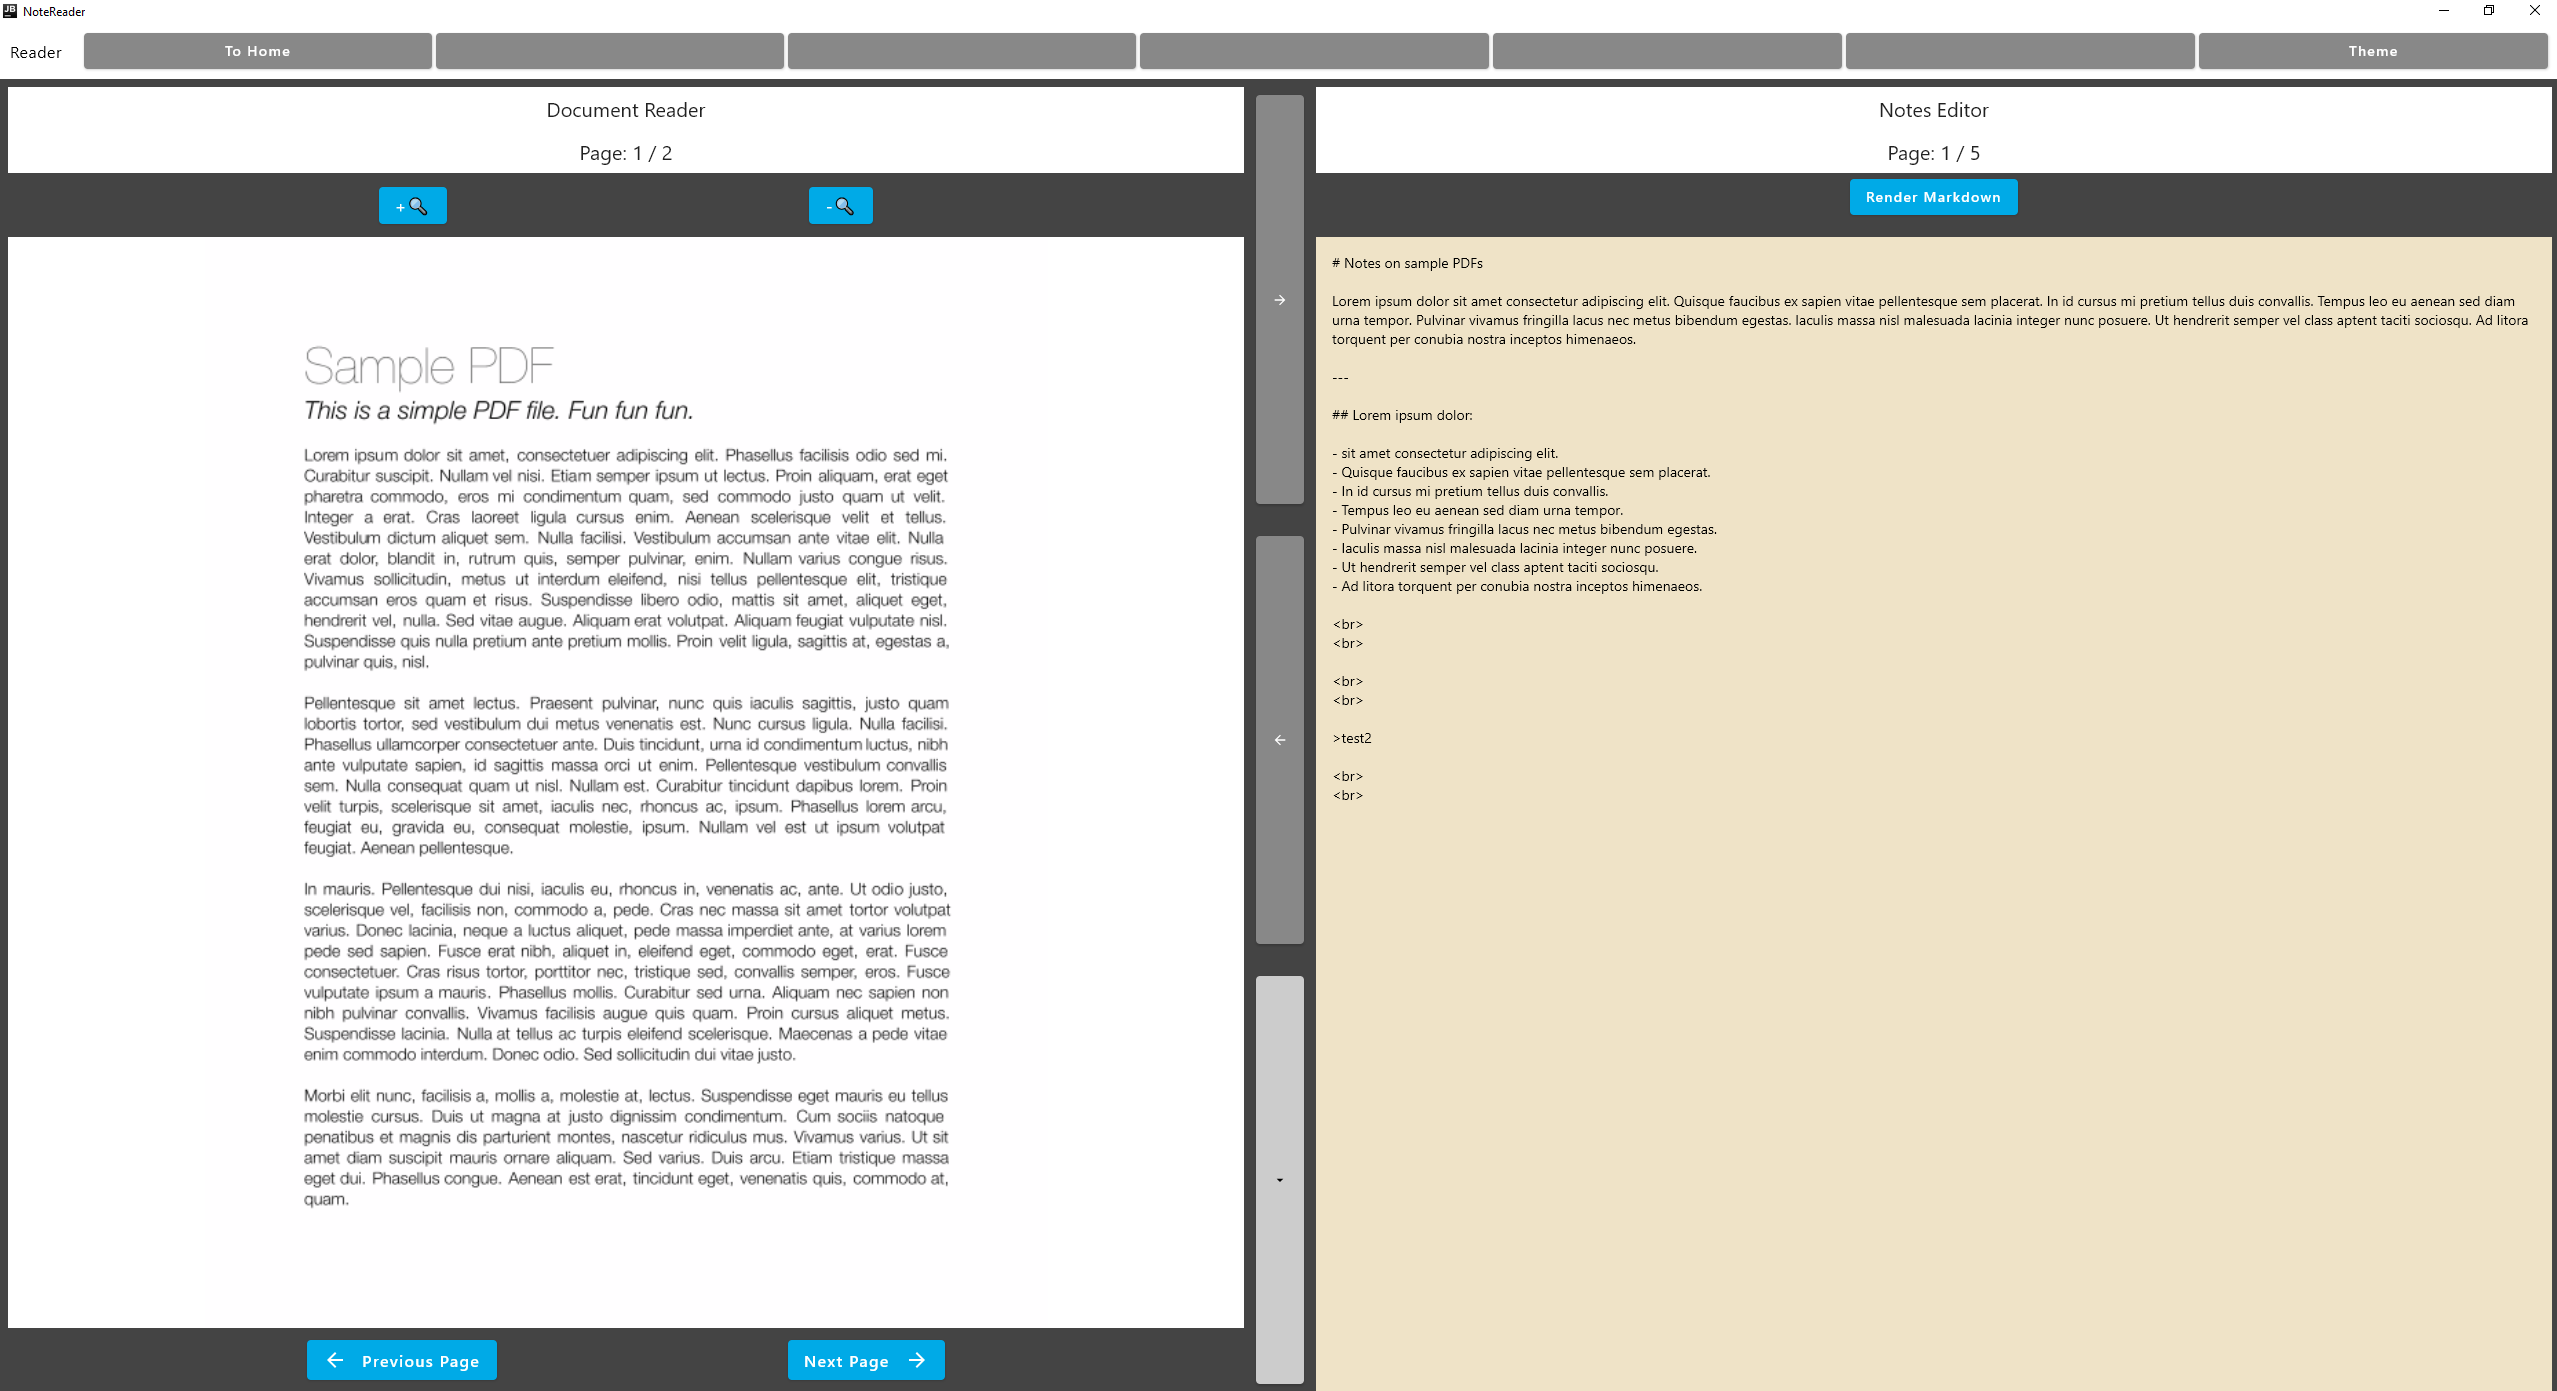
\includegraphics[width=1\linewidth]{image.png}
    \caption{Reader Page}
    \label{fig:reader}
\end{figure}


\begin{figure}
    \centering
    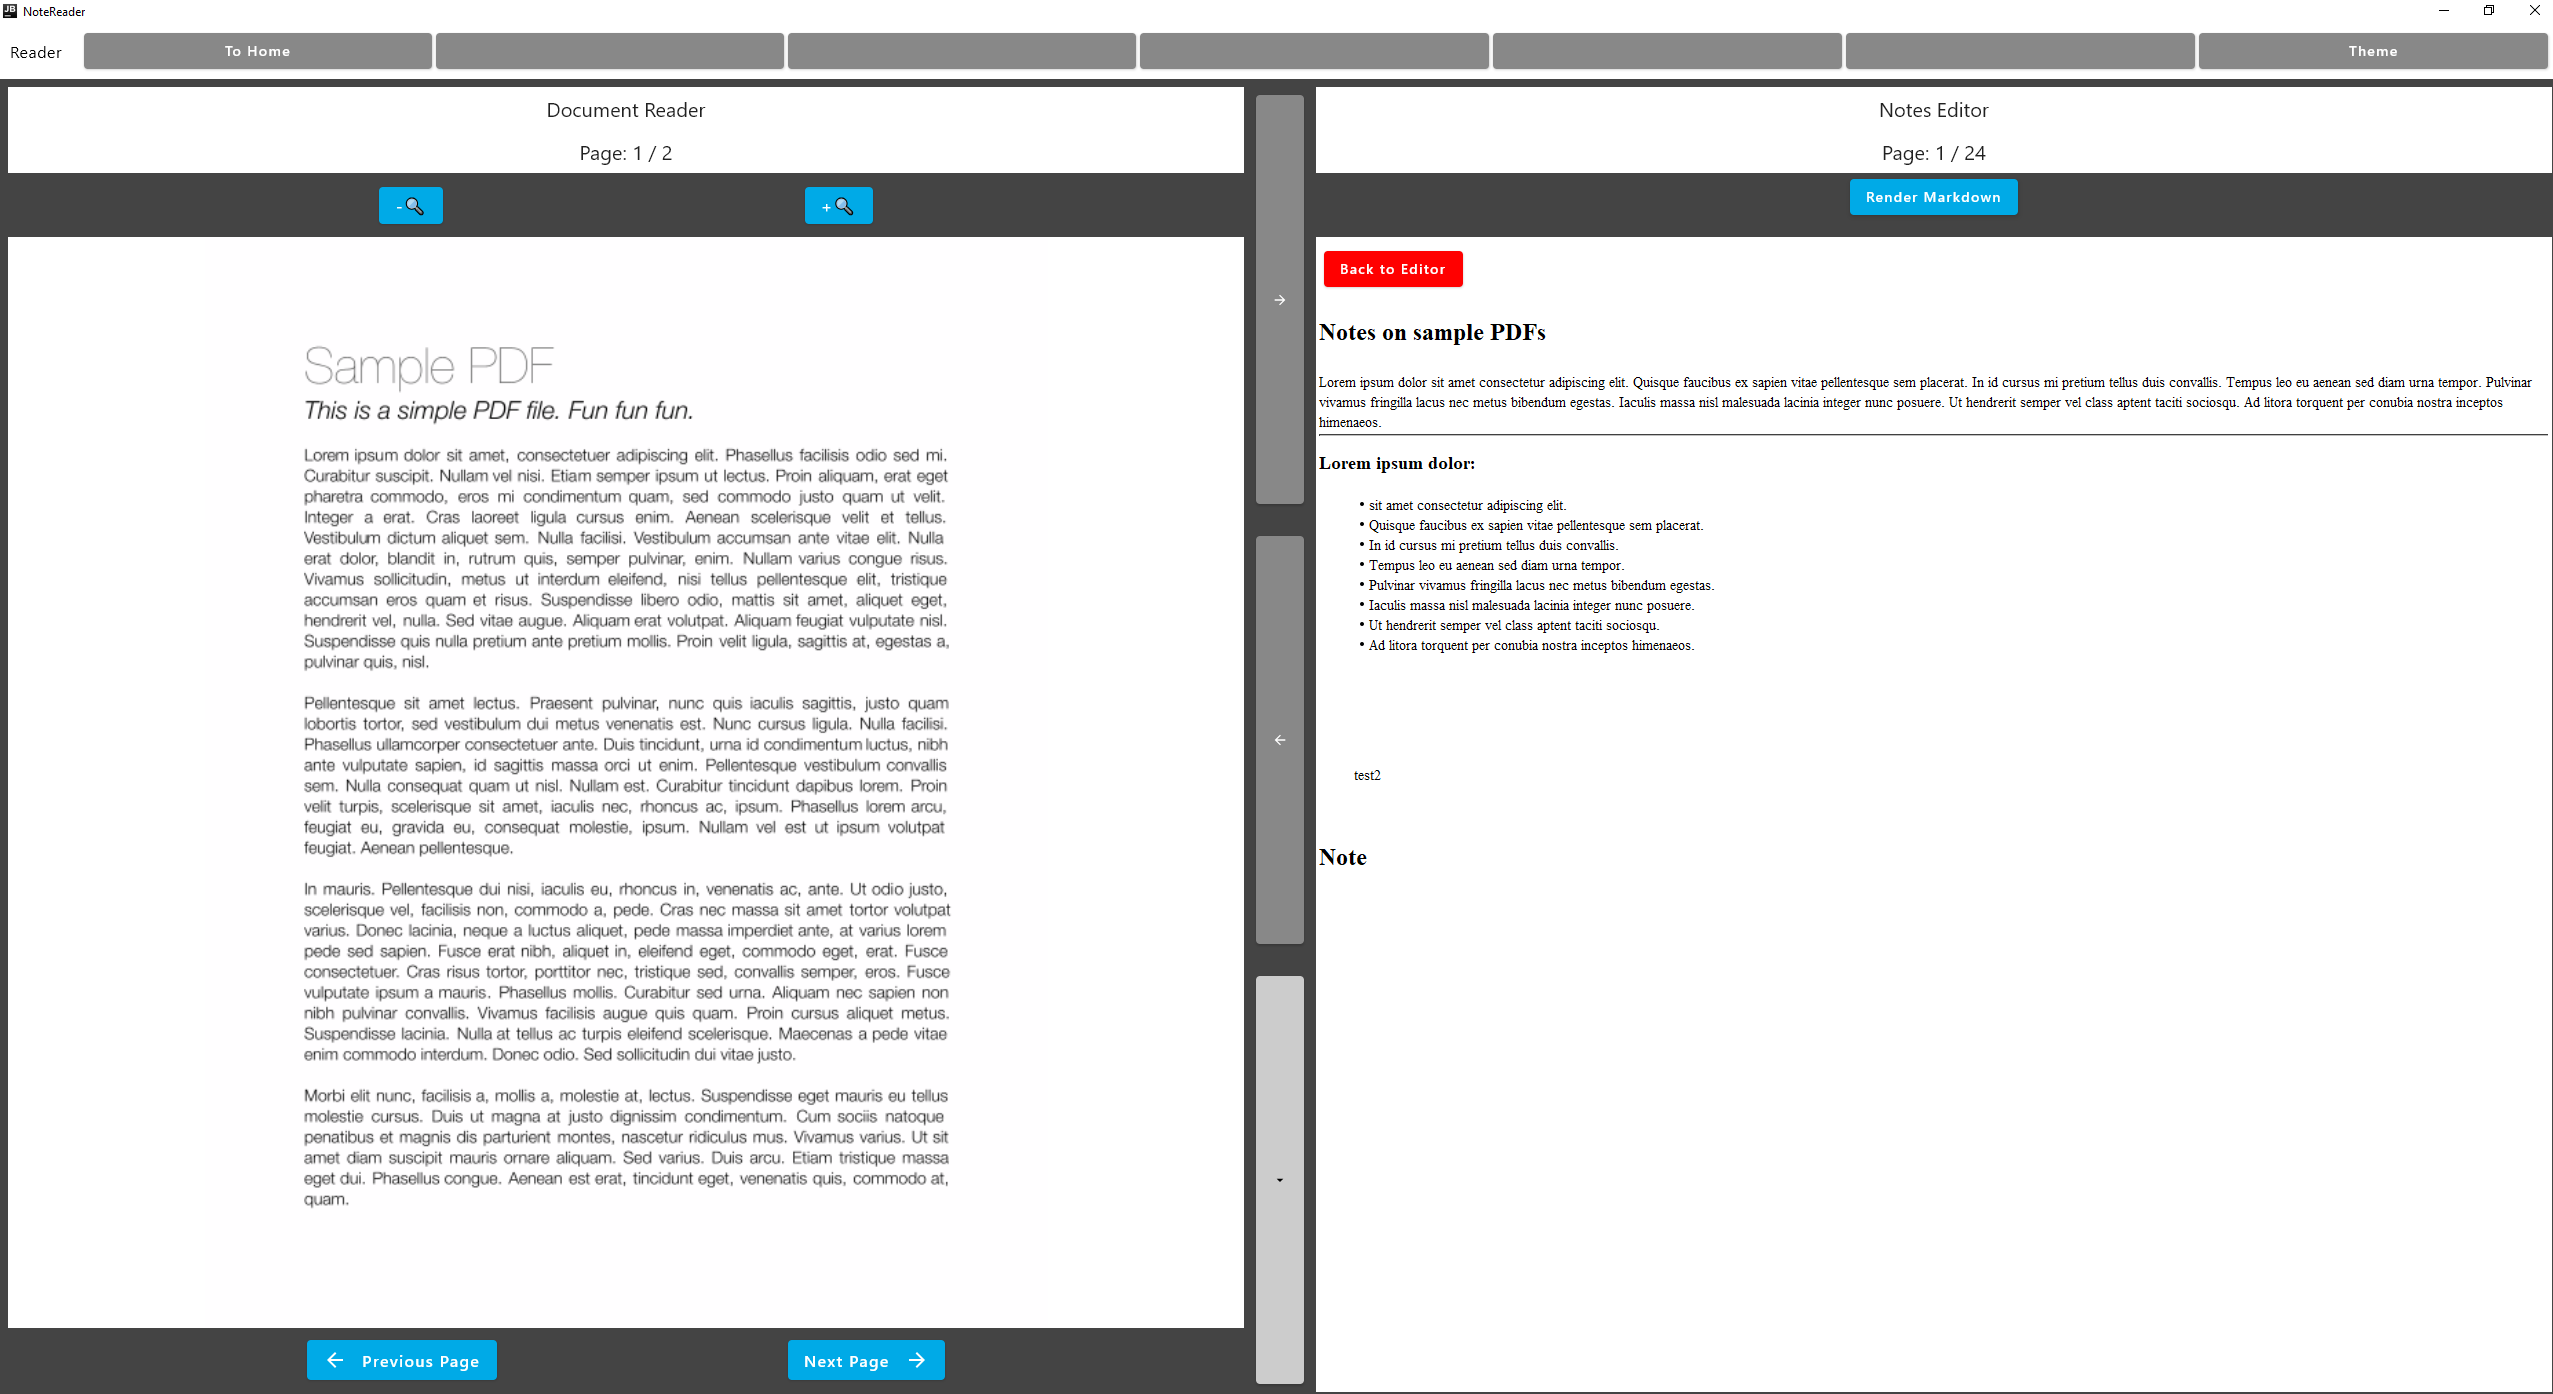
\includegraphics[width=1\linewidth]{Figures/image2.png}
    \caption{Markdown View}
    \label{fig:mdView}
\end{figure}

\begin{figure}
    \centering
    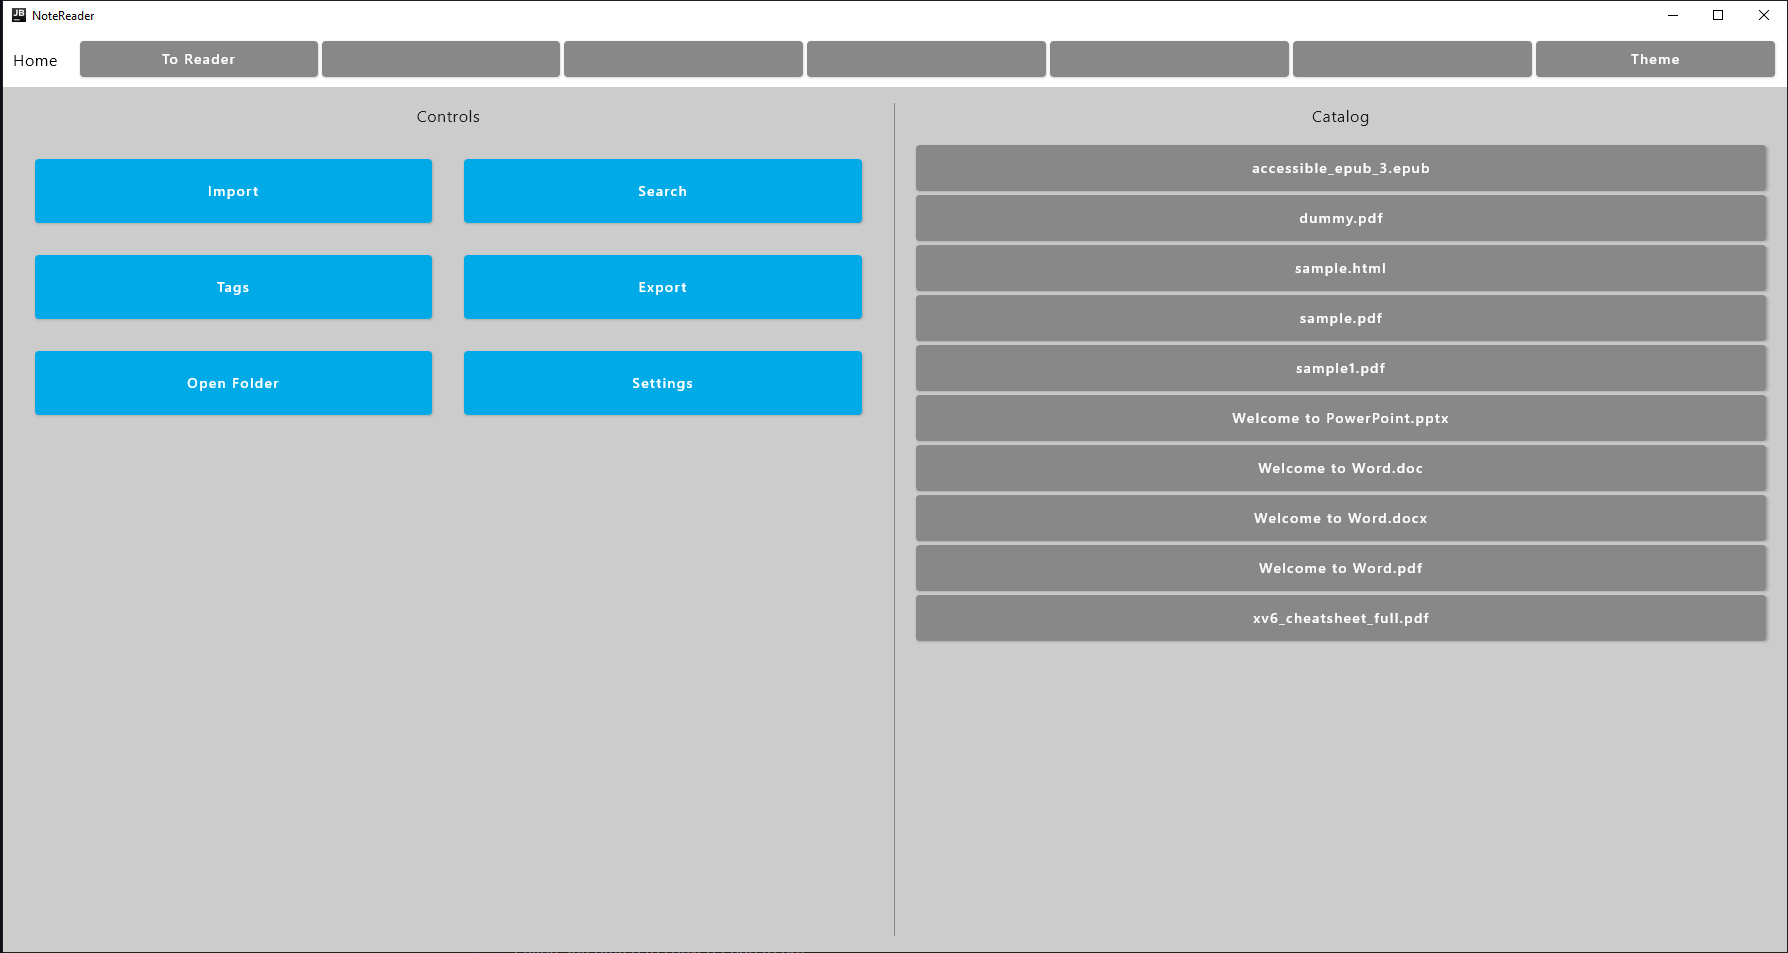
\includegraphics[width=1\linewidth]{Figures/image3.png}
    \caption{Home Screen}
    \label{fig:home}
\end{figure}

\begin{figure}
    \centering
    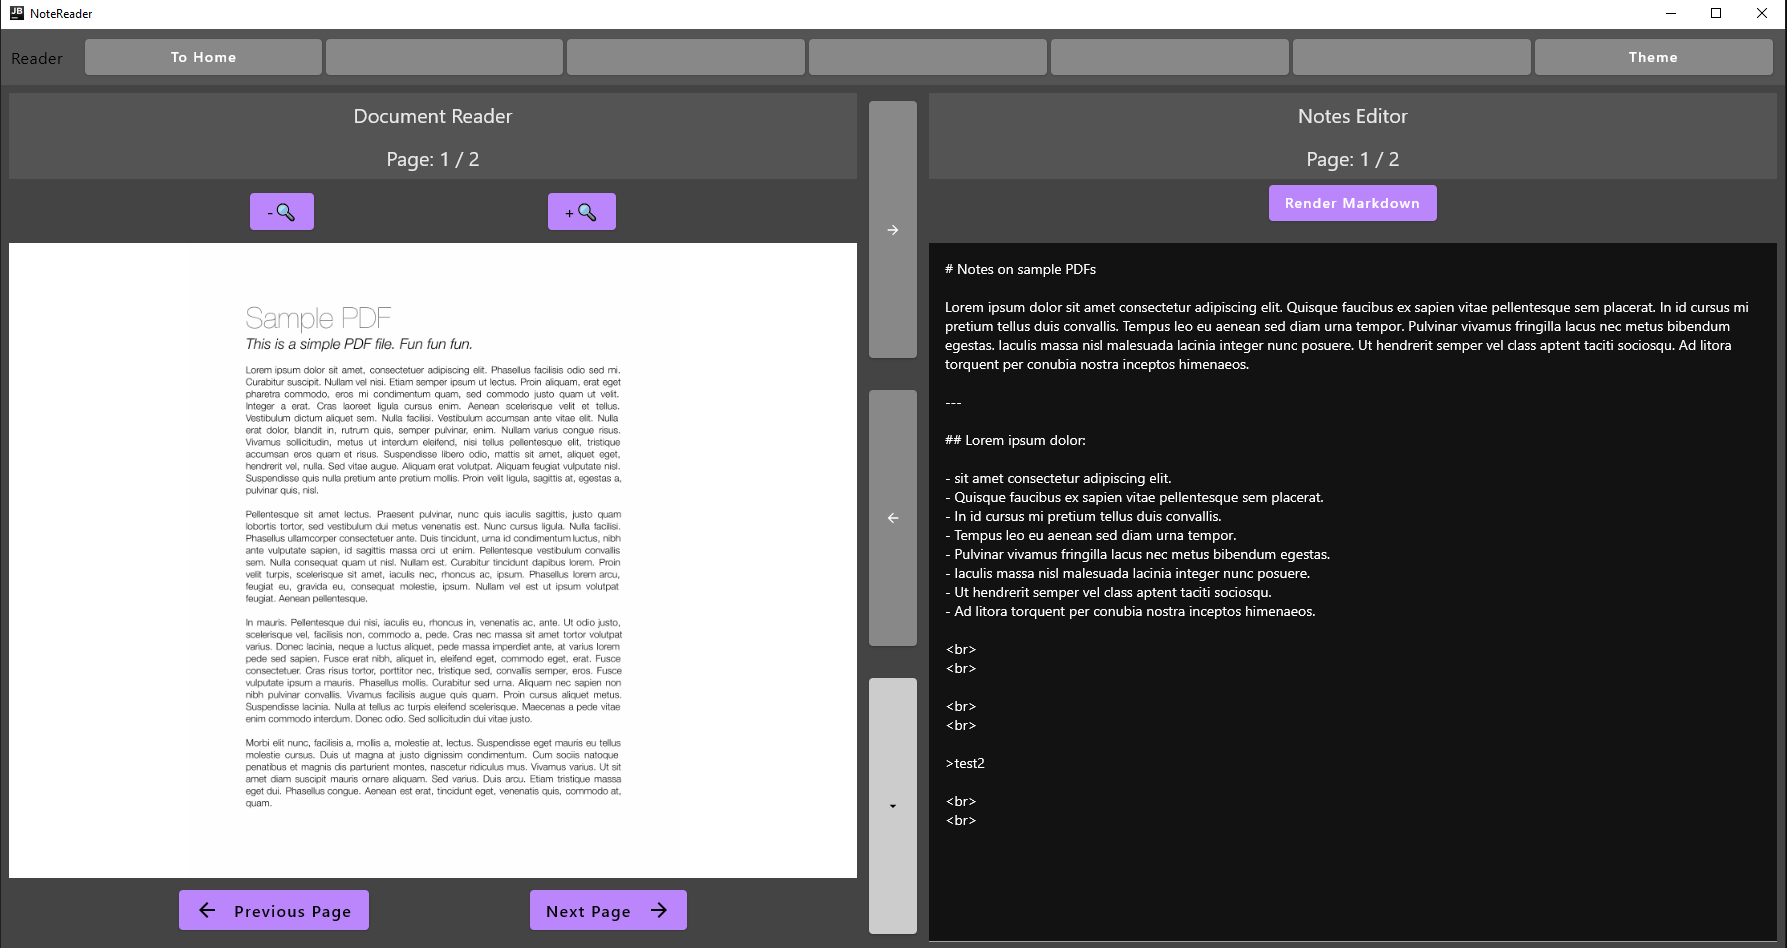
\includegraphics[width=1\linewidth]{Figures/image4.png}
    \caption{Dark Mode}
    \label{fig:dark}
\end{figure}

\subsubsection{Evolution of the Design and Lessons Learned}

The design of NoteReader evolved significantly over the course of development, shaped by technical constraints, time limitations, and practical insights gained through implementation. The foundation of the project however, split-view note taking, document integration, and plain-text note portability remained constant.

One of the most prominent evolutions was the architectural strategy for handling document rendering. The original goal was to have have native support for each format. This approach was determined to be impractical for a prototype. Instead, a fallback architecture was introduced: all supported document types were converted to PDF at runtime and rendered using a unified PDF renderer. This preserves the project's core requirement of true-to-intent document rendering, while simplifying implementation.

The scope of the project also shifted to emphasize core functionality. While the initial vision included synchronization, tagging and searching, and full multiplatform support, these features were pushed back to a later development cycle in order to focus on delivering a robust and usable Minimum Viable Product. Emphasis was placed on ensuring the design was fully modular, with string architecture to ensure these features could be integrated in future iterations. 

One of the most important lessons learned was the importance of adaptability in software projects. Various difficulties including framework maturity, integration complexity, and time management all influenced the project's direction. Attempting to strictly follow the original implementation plan would have made it difficult to deliver a completed product. The deferral of some requirements allowed the primary vision of the application to be maintained in the first iteration of the product, while preparing to implement those requirements in future. 


% In December of last year, when writing the first version of the report, in Chapter 4 you came up with your original solution approach. On it, you presented (i) the architecture of your solution, (ii) your list of use cases, (iii) a risk assessment, (iv) a methodology to develop your solution approach, (v) your implementation schedule, (vi) your evaluation plan and (vii) some prototype of the resulting product. From January to April you have been developing your solution approach. Along the way you have encountered difficulties (the ones listed in Section 5.1) which might have modified your original plan so that you can come up with an actual developed project.

% This section is effectively the production of "as built" specification where you compare your original design to the final finished project. Please go section by section (the ones listed from (i) to (vii) in the last paragraph. For each section, enumerate any difference between the original design and the final project, and justify the difficulty forcing you to make such this change. Do not fret if some of these changes are radical, what is important here is that there is a clear rationale for changes made.

 % Actual Implementation

\chapter{Testing and Evaluation}
\label{chap:eval}
\lhead{\emph{Project Testing}}

To validate the effectiveness of the NoteReader application, a comprehensive testing process was conducted. A variety of sample files in different formats were used to assess the system’s ability to meet its functional and non-functional requirements. These files included PDFs, DOCX, PPTX, EPUB, and HTML documents, and enabled rigorous evaluation of file parsing, rendering fidelity, and performance \ref{fig:sample_files}.


\section{Requirements}

    \subsection{Functional Requirements}
            \subsubsection{
            The system shall provide a split-view interface to allow users to view documents and take notes simultaneously}
            \textbf{Status: Fulfilled}   \newline
            The application successfully implements a split-view interface, where the document is displayed in the left pane and a markdown-compatible note editor appears in the right pane. \ref{fig:notereader_twopane}.
            
            \subsubsection {
            The system shall support the import and display of PDF, EPUB, DOCX, and PPTX files}            
            \textbf{Status: Fulfilled}   \newline
            The application supports a wide range of file types including PDF, DOCX, DOC, PPTX, EPUB, and HTML. These formats were selected based on their prevalence in academic environments and have been verified to load and render successfully and true to intent.
            
            \subsubsection {
            The system shall allow users to link notes to specific pages or sections of the source document.}            
            \textbf{Status: Fulfilled}  \newline
            The system correctly associates notes with specific pages of the source document. Each note is saved in a file named to reflect its corresponding page number, enabling automatic retrieval and display when users navigate to a particular page.
            
            \subsubsection {
            The system shall support searching and filtering of notes and documents using tags, keywords, and categories.}
            \textbf{Status: Not Fulfilled}  \newline
            This functionality was not implemented due to time constraints and has been deferred to future development cycles.
            
            
            \subsubsection {
            The system shall support exporting notes in plain text format for use in other applications.}
            \textbf{Status: Fulfilled}  \newline
            All notes are stored in markdown format (.md), enabling seamless export to and reuse in third-party applications such as Obsidian.
            
            
            \subsubsection {The system shall enable users to sync notes to cloud storage providers like GitHub using version control.}
            \textbf{Status: Not Fulfilled}  \newline
            Version-controlled synchronization using platforms like GitHub was intended but not implemented due to limited development time.

            
            \subsubsection {The system shall allow users to tag and categorize notes for efficient organization and retrieval.}
            \textbf{Status: Not Fulfilled}  \newline
            Although planned, tagging and categorization features were not developed in this phase of the project.
            


    \subsection{Non-Functional Requirements}
        \subsubsection { Performance: The system shall load and display documents without noticeable wait times on standard modern devices.}
        \textbf{Status: Partially Fulfilled}
        This Requirement has been partially fulfilled. PDF files are very quick to load, but the requirement to convert other document types can result in noticeable wait times. EPUB is especially long with the sample document taking approximately 5 seconds to load an ebook with 115 pages. 

        Once the document is converted however, it is very quick to navigate between pages. Pagination and lazy loading was implemented to ensure the impact on memory resources is kept to a minimum and ensure good performance. 


        \subsubsection { Usability: The user interface shall be intuitive, with clear user experience flows. }
        \textbf{Status: Fulfilled}

        This requirement is slightly more subjective, though I did design the application with this in mind, and would consider it to have been fulfilled. 

        I implemented the program in a manner which requires as few clicks as possible to enter a file. importing a document is as simple as selecting "import", then selecting the name of the document. 

        While in the reader view, The left pane shows the document, while the right shows the note taking window. The note taking window is coloured with a yellow tint, to evoke the thought of a traditional sticky note, so the purpose of the pane is immediately clear. 

        Buttons are large, and have icons that indicate their purpose, such as a magnifying glass for zooming. 


        \subsubsection { Scalability: The system shall support large document files (over 25mb), and offer alternative synchronization methods for these files. }
        \textbf{Status: Deferred}
        Although large files can be imported, advanced synchronization strategies for large datasets (e.g., LFS for Git) are not yet implemented and remain a future goal.

        
        \subsubsection { Portability: The system shall support cross-platform functionality on Windows, macOS, Linux, and mobile devices.}        \textbf{Status: Not Yet Fulfilled}
        While the application has not yet been deployed on multiple platforms, it is architected using Kotlin Multiplatform, enabling straightforward extension to additional targets in future iterations.

    
        \subsubsection { Reliability: The system shall gracefully handle unexpected crashes to prevent data loss by saving notes in real-time and automatically restoring the last working state upon restart.}
        \textbf{Status: Fulfilled}
        All notes are saved in real time as the user edits them.
        A persistent application state is maintained using a JSON file, which is read on application launch to restore the last session \ref{fig:state_json}

         
        \subsubsection { Maintainability: The system shall be modular to allow for easy updates and addition of new features.}
        \textbf{Status: Fulfilled}

        The application employs a Model-View-Controller (MVC) architecture, supporting clean separation of concerns. 
        
        Views are built in Compose, allowing individual components to be replaced or extended with minimal coupling. 
        
        New document format support can be easily added by inserting appropriate logic modules into the existing flow.
        

\begin{figure}
    \centering
    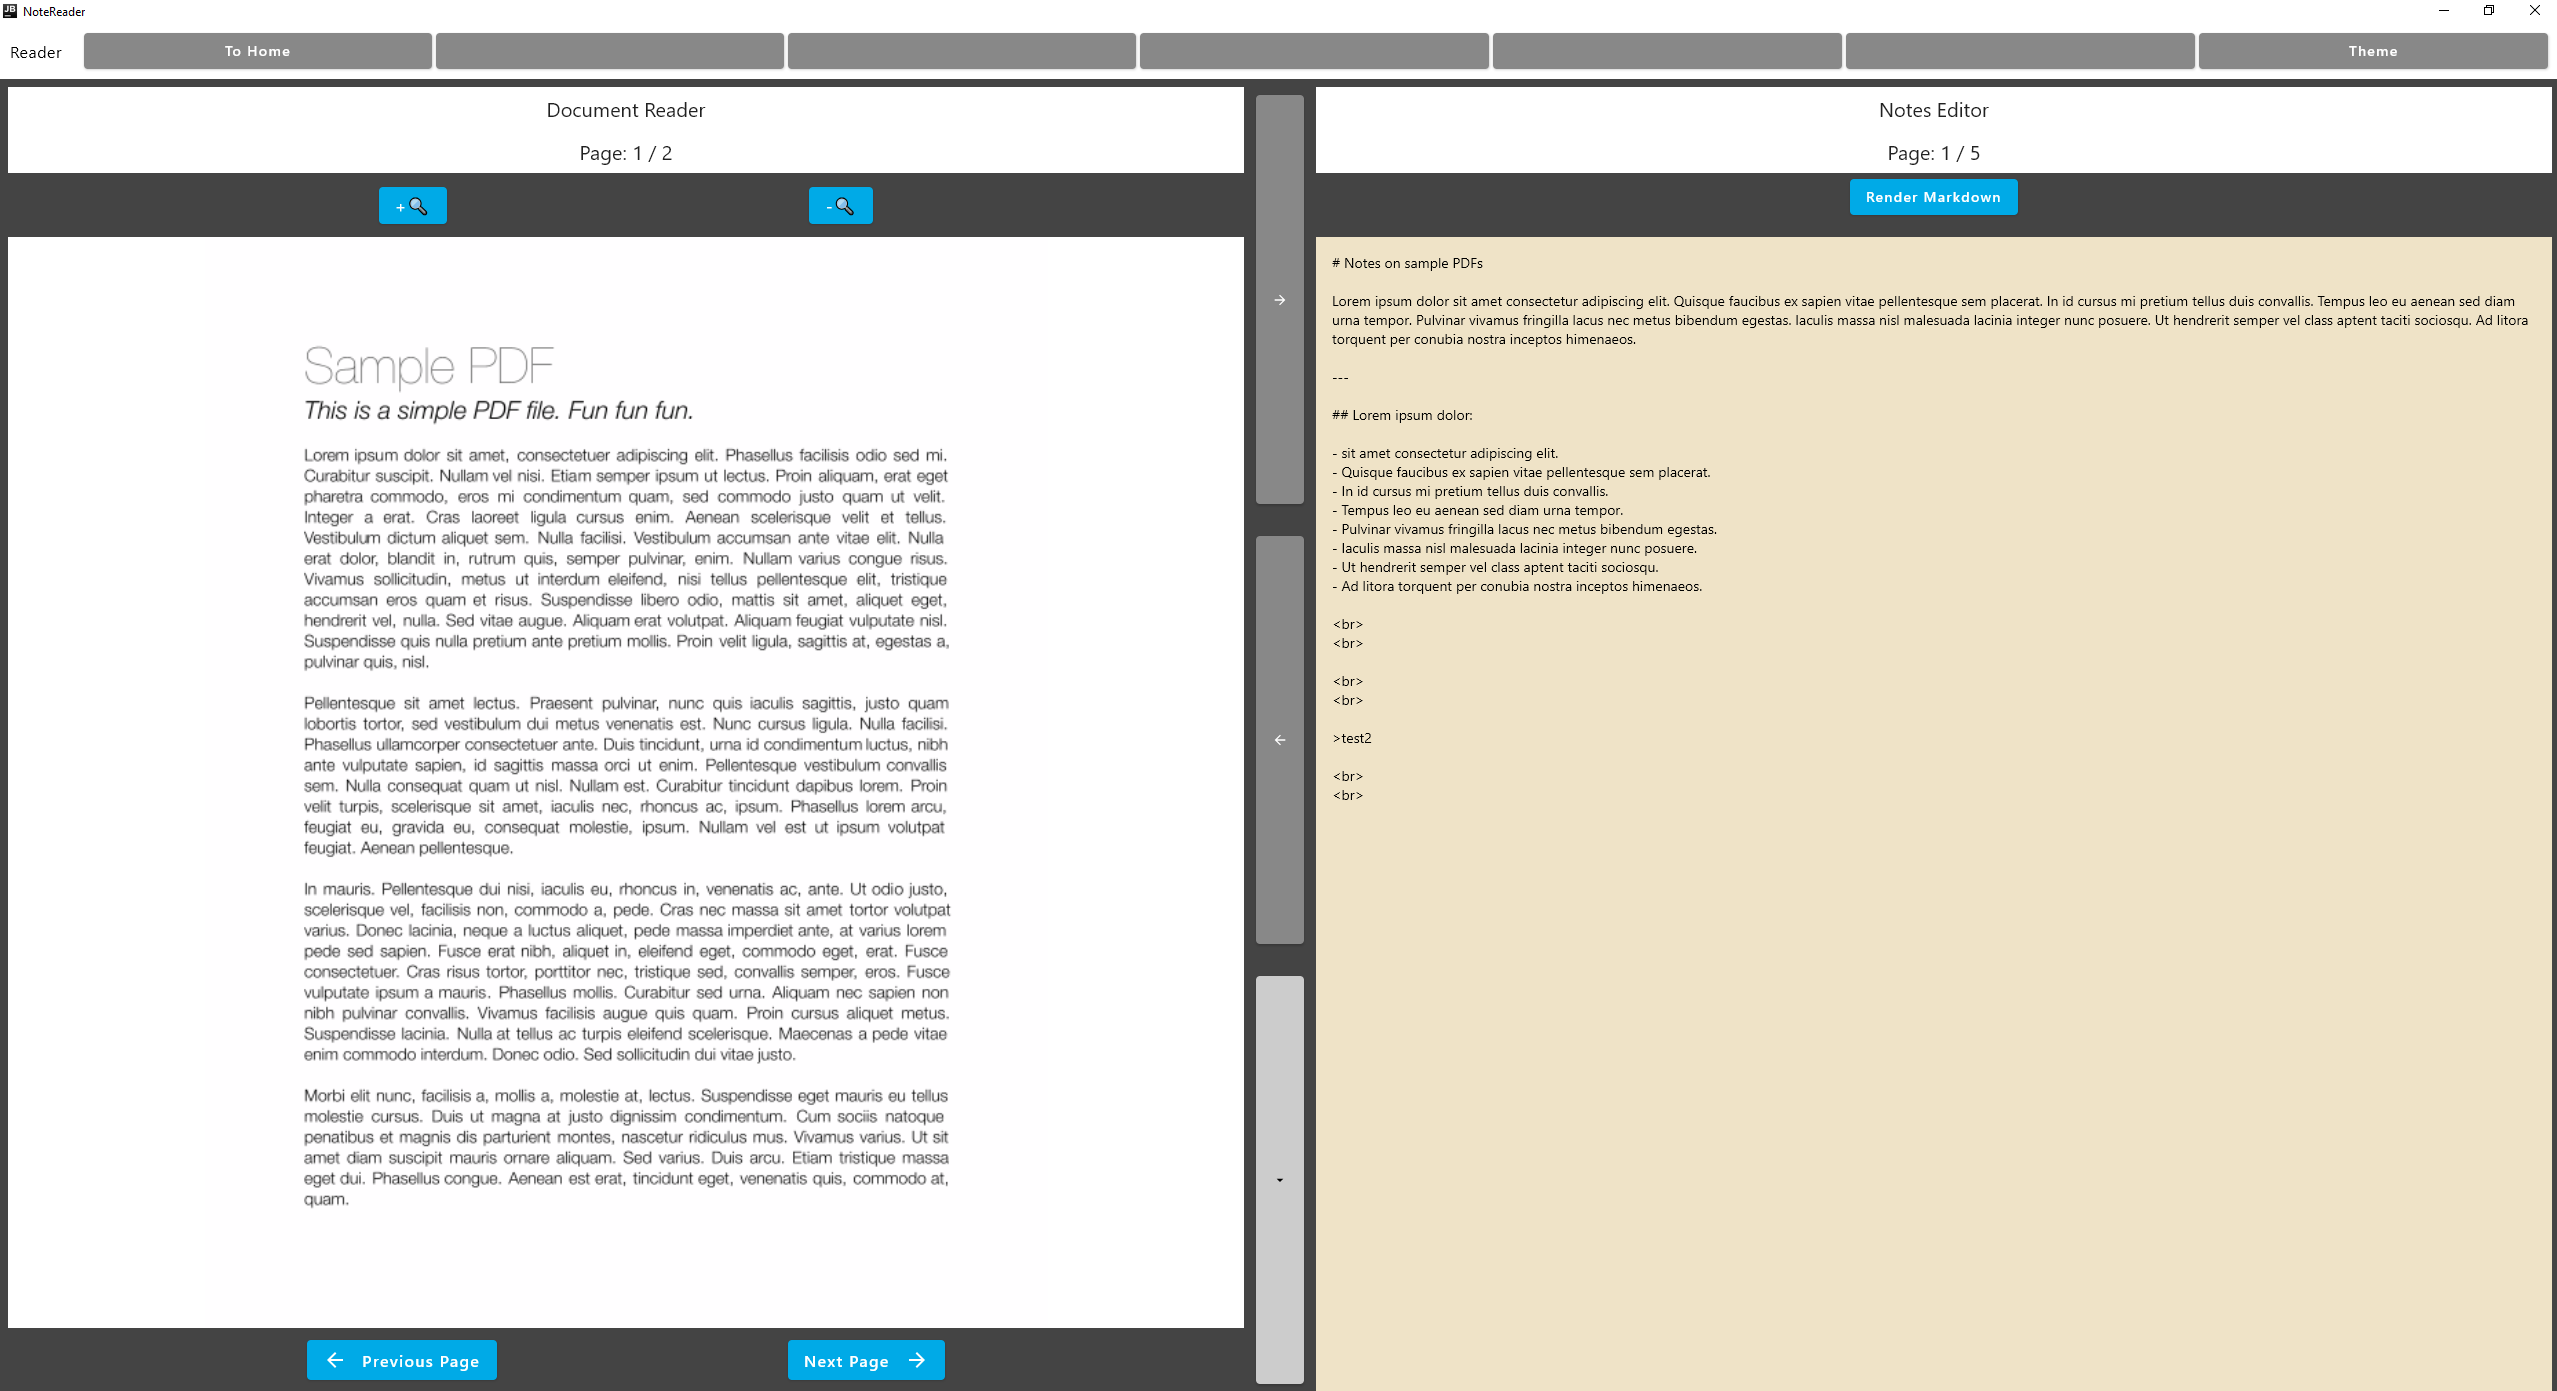
\includegraphics[width=1\linewidth]{image.png}
    \caption{A screenshot of the NoteReader Application, showing the two pane layout}
    \label{fig:notereader_twopane}
\end{figure}    

\begin{figure}
    \centering
    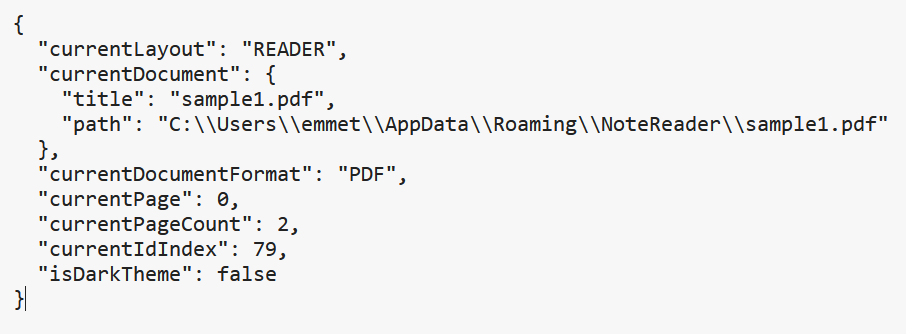
\includegraphics[width=1\linewidth]{state_json.png}
    \caption{Sample Program State in Json Format}
    \label{fig:state_json}
\end{figure}

\begin{figure}
    \centering
    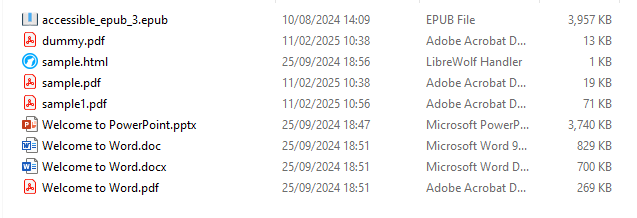
\includegraphics[width=1\linewidth]{sample_files.png}
    \caption{Sample Files used for testing}
    \label{fig:sample_files}
\end{figure}

% The goal of this chapter is an objective evaluation of the final system. The evaluation must be quantitative and not qualitative. You may perform qualitative evaluation but this should not form the basis of the main conclusions you derive from the evaluation. This evaluation, where possible, should be comparative, i.e. you should evaluate your system against a commercially available system and/or system detailed in a research publication. You should demonstrate operational testing of the project using real or contrived data sets to evaluate aspects of the project not encompassed in the software testing (e.g. quantify how well does your project achieved the overall goal). 
% \begin{itemize}
%     \item For software based projects this will include, but should not be limited to, evaluation of non-functional requirements.
%     \item For infrastructural projects this testing should include system/network KPI analysis.
%     \item For analysis based projects (ML, malware or other) this may include model evaluation or YARA rule validation, for example.
%     \item For management projects, where software testing or infrastructure testing may not be in scope, the test process for the system is expected to be more rigorous and well described than a project incorporating significant development work.
% \end{itemize} 

% Some suggested sections (the nature of this chapter should be discussed in detail with your term 2 supervisor):

\section{Metrics}
% Identify and describe the metrics you used to evaluate your project. You should have identified some of these in the research phase report but will detail these as you progress through the design.

\begin{itemize}
    \item \textbf{Feature Completeness}: Whether each intended feature was implemented and functioned as expected during manual use.
    \item \textbf{File Compatibility}: Evaluation of whether a variety of common document formats (PDF, DOCX, EPUB, PPTX, HTML) could be opened, rendered, and navigated.
    \item \textbf{Stability and Recovery}: Observations of the application's behaviour when reopened after closing mid-session, including state persistence, and real time saving of notes.
    \item \textbf{Document-to-Note Linking Accuracy}: Inspection of whether notes correctly reloaded for their associated page, and validating that files are created and sorted appropriately. 
\end{itemize}

These observational metrics provided a practical basis for assessing whether NoteReader met its intended goals and provided a usable experience for real-world document annotation workflows.



\section{System Testing}
% Describe the experimental setup for each metric, and how you obtained the measurements. Describe the inputs for each experiment

System testing was conducted manually, using a range of sample files selected to represent typical academic study materials. The goal was to validate the system’s ability to import, render, and annotate documents across a variety of formats. The following test process was followed:

\begin{itemize}
    \item \textbf{Document Import and Rendering}: Sample files (PDF, EPUB, DOCX, PPTX, HTML) were imported to check if they rendered correctly in the split-view layout. Each file was inspected for formatting integrity and legibility.
    \item \textbf{Note Creation and Retrieval}: Notes were created for specific pages, then navigation was tested to confirm that the correct note appeared when returning to that page.
    \item \textbf{Session Persistence}: The program was closed mid-session and reopened to test whether the last viewed document and notes were restored successfully. Crashes were simulated by ending execution of the program directly in the Android Studio IDE. 
    \item \textbf{File System Inspection}: The folder structure and file output were manually verified to confirm that notes were stored in plain-text markdown format and logically organized per document.
\end{itemize}

While these tests did not produce numeric results, they provided confidence that core functionality worked as intended under normal usage conditions.

\section{Results}
% Summarise the output data, and the statistical or other techniques to deduce your results. Summarise your results, including tables or graphs as appropriate with a brief description of each. here possible, compare your results with other products/systems. Identify any possible threats to the validity of your results, and discuss each briefly here (you will discuss in more detail in the next chapter).

The manual testing process confirmed that the core features of NoteReader function as expected across a range of sample documents. Below is a summary of observed results:

\begin{itemize}
    \item \textbf{File Compatibility}: All tested formats PDF, DOCX, PPTX, EPUB, and HTML were successfully rendered using the PDF conversion pipeline. Formatting was preserved in all cases.
    \item \textbf{Note Linking}: Notes were correctly saved per page and reloaded without error. 
    \item \textbf{State Restoration}: On restarting the application, the previous session's document and page state were restored, confirming that persistence was functioning as designed. when simulating crashes, all notes were verified to have saved correctly. 
    \item \textbf{Interface Stability}: In the final version no crashes were encountered during normal use.
\end{itemize}

\subsection{Limitations}
\begin{itemize}
    \item A lack of automated testing may lead to blind spots over time. Manual testing was appropriate for the graphical elements of the application, but subsequent development cycles should focus on unit testing as a priority. 
    \item Testing was conducted only on two devices (Windows 10 and Windows 11).
    \item No formal load or performance testing was conducted. While considerations were made to performance, such as the implementation of lazy loading and pagination, observations of responsiveness were subjective.
\end{itemize} % Testing
\chapter{Discussion and Conclusions}
\label{chap:conclusions}
\lhead{\emph{Discussion and Conclusions}}
% In this chapter, you should expand upon (and initially reflect upon) the discussion and conclusion of the research phase of the project. The expectation here is that you should discuss the results presented in the previous evaluation section of the project in their totality (i.e. as a whole) from which you will then draw clear conclusions both on the quantitative and qualitative aspects of the overall project. This chapter should be a about 2000 words long (5 pages of text - 1600 words of discussion and 400 words of conclusion). This may vary depending on quality. The conclusion section of this report should conclude the project.

% Some suggested sections (the nature of this chapter should be discussed in detail with your term 2 supervisor):

\section{Solution Review}
% Discuss how well your solution solves the problem, based on your results from the evaluation chapter.
The final implementation of NoteReader addresses the core problem identified at the beginning of the project: the lack of an integrated solution that treats both document reading and note-taking as first class features.

The completed NoteReader prototype delivers a focused and practical solution to the challenge of fragmented note-taking and document reading workflows.  

The application successfully provides a split-view interface that allows users to read documents and take notes simultaneously, preserving contextual relevance and reducing cognitive load.

The system support all targeted document types, with an architecture designed to expand support to further formats. It supports document page to note linking and session persistence. While features like search, tagging, and Git synchronization were not completed, the application architecture supports their future inclusion.

While certain requirements were deferred to later development cycles, the project acts as a solid proof of concept, and illustrates the value of the core features. 

\section{Project Review}
% Discuss how well you addressed the project, and what you might do differently if you were to do it again. Make sure to identify how you handled any problems that arose during the project. Identify key skills that you learnt during the project, and clearly describe how you applied these, and how you might apply them differently if you were to do a similar project.

The project was approached using an agile methodology, structured around iterative development in five adjusted sprints. Although the original plan envisioned six evenly distributed sprints, difficulties encountered, particularly in areas involving document rendering, required adjustments to the original strategy.

Key challenges included the immaturity of the Kotlin Multiplatform framework, limitations in third-party libraries, and the time-intensive nature of converting diverse document types while preserving author intent. 

If this project were to be undertaken again, earlier identification of technological limitations would have enabled a more realistic scope. A stronger focus on UI prototyping and automated testing could also have improved development efficiency and user confidence.

Throughout the project, a number of valuable skills were developed:

\begin{itemize}
    \item \textbf{Cross-platform development}: Learned how to structure shared logic in Kotlin Multiplatform, and abstract platform-specific implementations.
    \item \textbf{Interface design and user experience}: Applied UX design principles to build an intuitive and minimalist interface.
    \item \textbf{Document processing and conversion}: Gained hands-on experience with libraries such as Apache POI, PDFBox, and external tools for document conversion.
    \item \textbf{State persistence and modular architecture}: Designed and implemented a maintainable file structure and session recovery mechanism.
\end{itemize}

These skills not only contributed to the successful delivery of NoteReader’s MVP but will be directly transferable to future software development projects that require cross-platform deployment, structured UI design, or file format interoperability.


\section{Conclusion}
% Enumerate the main conclusions you have got in terms of background, problem description and the solution approach you have come up with. Detail your primary and any secondary conclusions from your project.

This project set out to explore whether a unified application could bridge the gap between document reading and note-taking in a way that supports better organization, learning, and review. The investigation into current market tools revealed a recurring theme: fragmentation, platform lock-in, and poor contextual linking between notes and source materials.

NoteReader demonstrated a practical solution that merges document viewing and structured note-taking into a single interface. Core features, including split view layout, page specific note linking, plain text file storage, and persistent session state   were successfully implemented and validated through manual testing.

The primary conclusion is that the design approach enabled the delivery of a functional MVP with potential for further growth. 

Secondary, adopting cutting-edge frameworks (e.g., Kotlin Multiplatform) can accelerate innovation, but must be balanced against the increased risk of instability and limited ecosystem support.

NoteReader stands as a proof of concept that contextual, cross linked note taking is both feasible and desirable, and can serve to save time, prevent data loss and reduce cognitive load. 

\section{Future Work}
% Discuss any proposals for completion of the project, or for enhancements, or for re-design of your solution or software. Enumerate all the things you would have wanted to do should you have more time to work on this project.

While the project achieved a core Minimum Viable Product, there are several areas identified for further development and enhancement:

\begin{itemize}
    \item \textbf{Search and Tagging System}: Implementation of a tag-based and full-text search system for fast filtering of notes and documents remains a high-priority feature.
    \item \textbf{Git Integration}: Enable Git-based version control and synchronization to allow for cross-device usage and version history tracking of notes.
    \item \textbf{Cross-Platform Expansion}: Extend support to macOS, Linux, and mobile platforms using Kotlin Multiplatform’s shared logic model and Compose Multiplatform's UI capabilities.
    \item \textbf{OCR and Handwriting Support}: Add optical character recognition for image-based documents and enable stylus input for users who prefer handwritten notes.
    \item \textbf{User Customization}: Provide theme support, customizable keyboard shortcuts, and user settings for layout and accessibility.
    \item \textbf{Searchable Catalogue UI}: Build a graphical catalogue browser for easier navigation and visualization of stored documents and notes.
    \item \textbf{Improved EPUB Rendering}: Enhance rendering fidelity for EPUB files using more performant native libraries or better conversion processes.
    \item \textbf{Audio/Video Notes with Timestamps}: Allow users to take notes linked to specific timestamps during lecture recordings or media playback.
\end{itemize}

If more time and resources were available, these improvements would bring NoteReader closer to a fully featured application suitable for release and daily academic use. The current prototype serves as a solid foundation upon which these features can be gradually layered in a modular and maintainable way. % Discussion and Conclusion
\fi

%% ----------------------------------------------------------------
\label{Bibliography}
\bibliographystyle{IEEEtranN}  % Use the "IEEE Transaction" BibTeX style for formatting the Bibliography
\bibliography{Information/Bibliography}  % The references (bibliography) information are stored in the file named "Bibliography.bib"
\lhead{\emph{Bibliography}}  % Change the left side page header to "Bibliography"

%% ----------------------------------------------------------------
% Now begin the Appendices, including them as separate files

\addtocontents{toc}{\vspace{2em}} % Add a gap in the Contents, for aesthetics

\appendix % Cue to tell LaTeX that the following 'chapters' are Appendices

\chapter{Code Snippets}

\section{Early Prototyping}
Following are a number of small code snippets with basic implementation of some core features. This code is written in C\# using WPF, and is not intended for use in the final program. These are simply early explorations into the concepts. 
\newpage

\begin{figure}
    \centering
    \begin{lstlisting}
public void SaveCurrentMarkdown()
{
    var content = MarkdownEditor.Text;
    if (!string.IsNullOrWhiteSpace(content))
    {
        var filePath = Path.Combine(notesFolderPath, $"{CurrentPageIndex}.md");
        markdownHandler.SaveMarkdown(filePath, content);
        UpdateSaveStatus("Saved", false);
    }
}
    \end{lstlisting}
    \caption{An example of creating a notes markdown file, which uses the current page number as the name of the file, so it can be found when the page is re-opened. }
    \label{SaveCurrentMarkdown}
\end{figure}

\begin{figure}
    \centering
    \begin{lstlisting}
using VersOne.Epub;

public class EpubLoader
{
	public List<FlowDocument> LoadEpub(string epubPath)
	{
		var epubBook = EpubReader.ReadBook(epubPath);
		var contentFiles = epubBook.ReadingOrder.OfType<EpubLocalTextContentFile>().Select(chapter => chapter.Content);
		return ConvertToFlowDocuments(contentFiles, epubBook.Content.Images.Local);
	}
    private List<FlowDocument> ConvertToFlowDocuments(IEnumerable<string> contentFiles,
		IReadOnlyCollection<EpubLocalByteContentFile> images)
	{
		if (contentFiles == null || images == null)
			throw new ArgumentNullException("contentFiles or images cannot be null");

		var flowDocuments = new List<FlowDocument>();

		foreach (var content in contentFiles)
        
......... Specific Implementation omitted for brevity .........

			var htmlPanel = new HtmlPanel();
			htmlPanel.Text = htmlDoc.DocumentNode.OuterHtml;
			document.Blocks.Add(new BlockUIContainer(htmlPanel));

			flowDocuments.Add(document);
		}

		return flowDocuments;
	}
    \end{lstlisting}
    \caption{An example approach of displaying an EPUB file in a HTML renderer}
    \label{EPUB to HTML}
\end{figure} % Appendix A
\chapter{Wireframe Models and Diagrams}
\label{Wireframes}

\begin{figure}
    \centering
    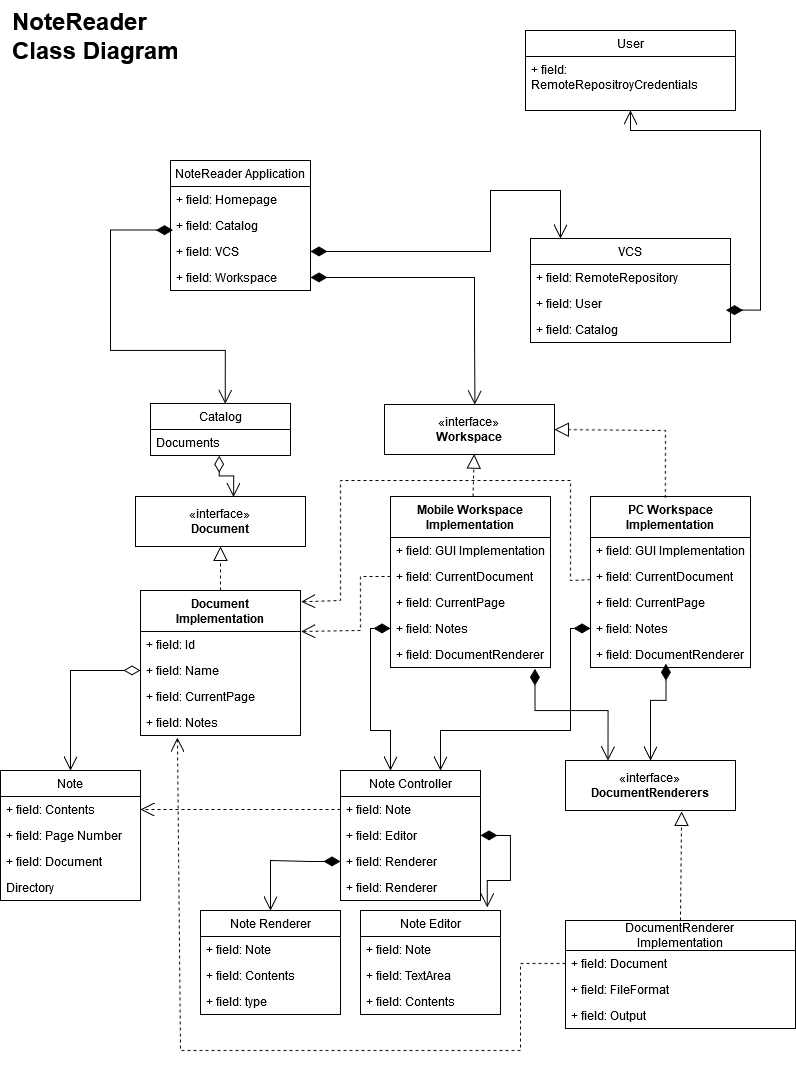
\includegraphics[width=1\linewidth]{Figures/Class Diagram.drawio(2).png}
    \caption{Application Class Diagram, Illustrating high level overview of Architecture}
    \label{fig:CD}
\end{figure}

\begin{figure}
\centering
\subfigure[NoteReader in Notes Editing Mode]{\label{fig:NoteReaderMock1}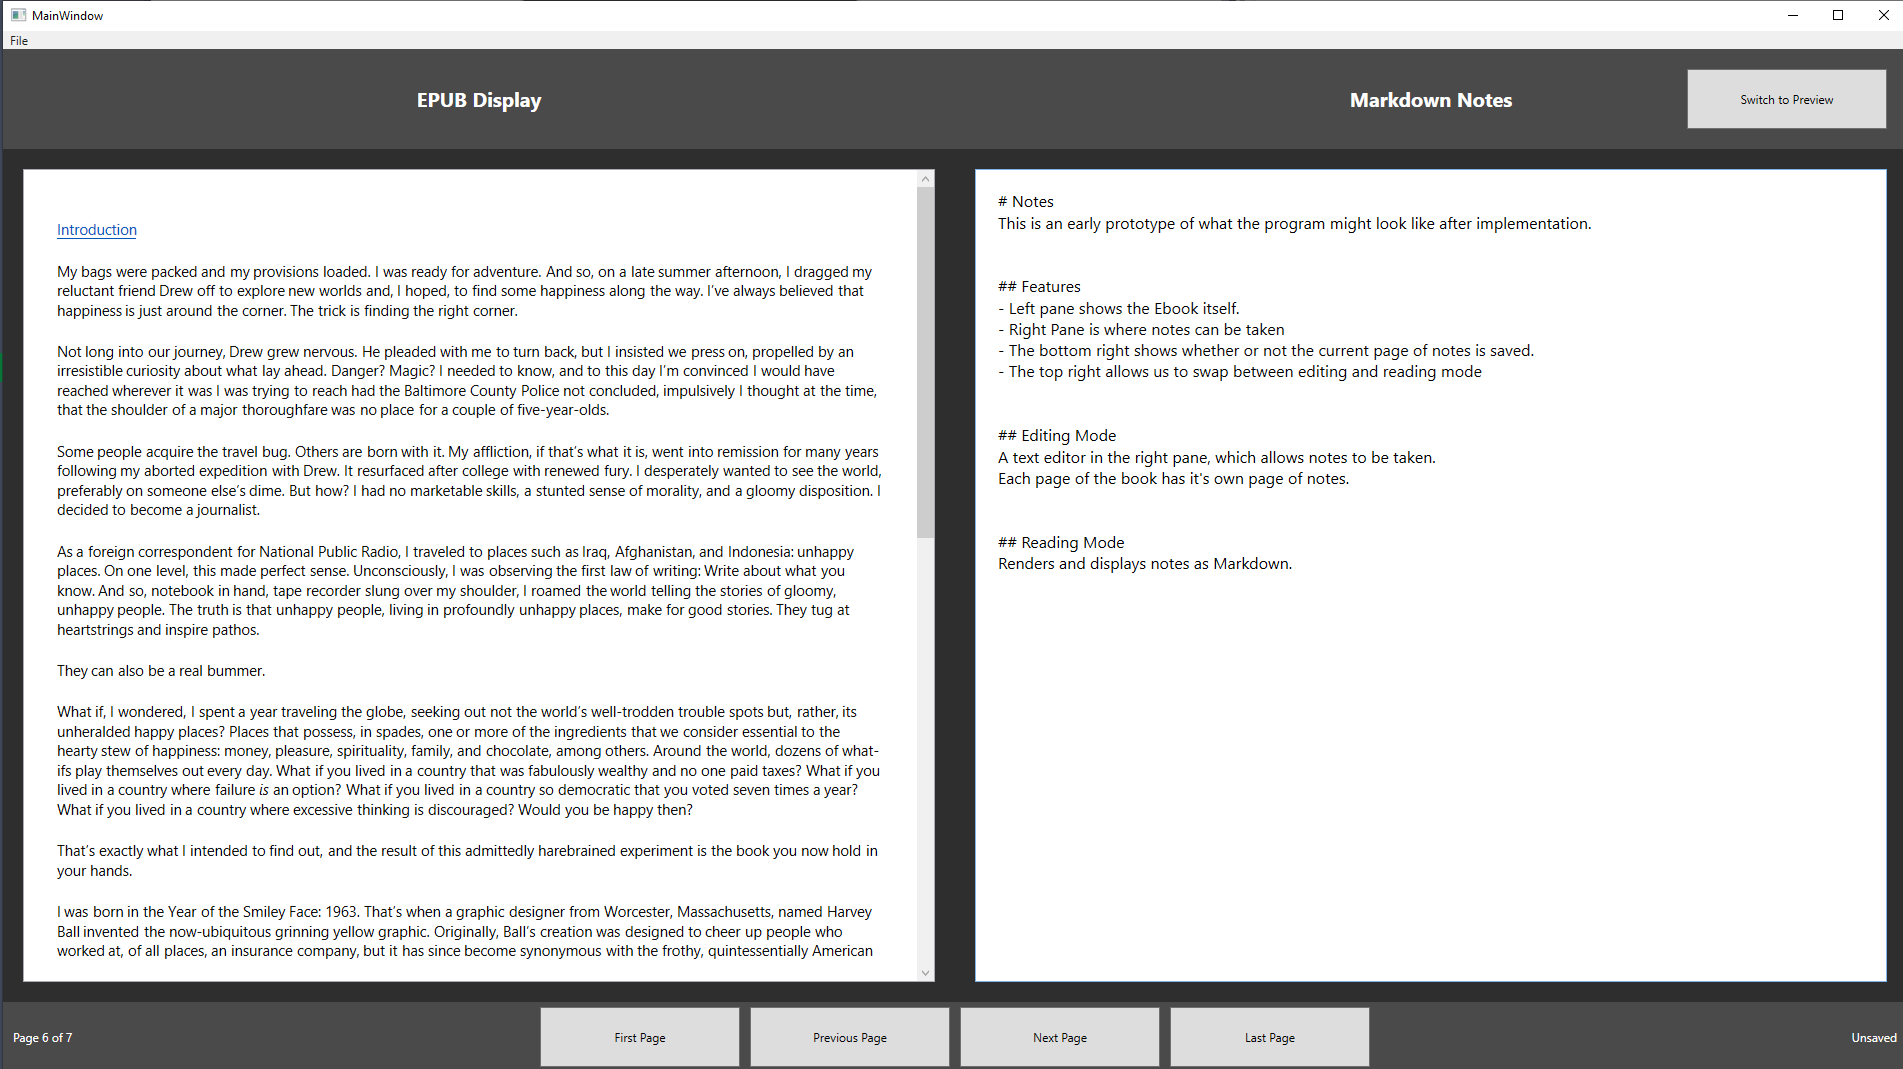
\includegraphics[width=1\textwidth]{Figures/Screenshot 2024-12-14 204141.png}}
\subfigure[NoteReader in Notes Rendering Mode]{\label{fig:NoteReaderMock2}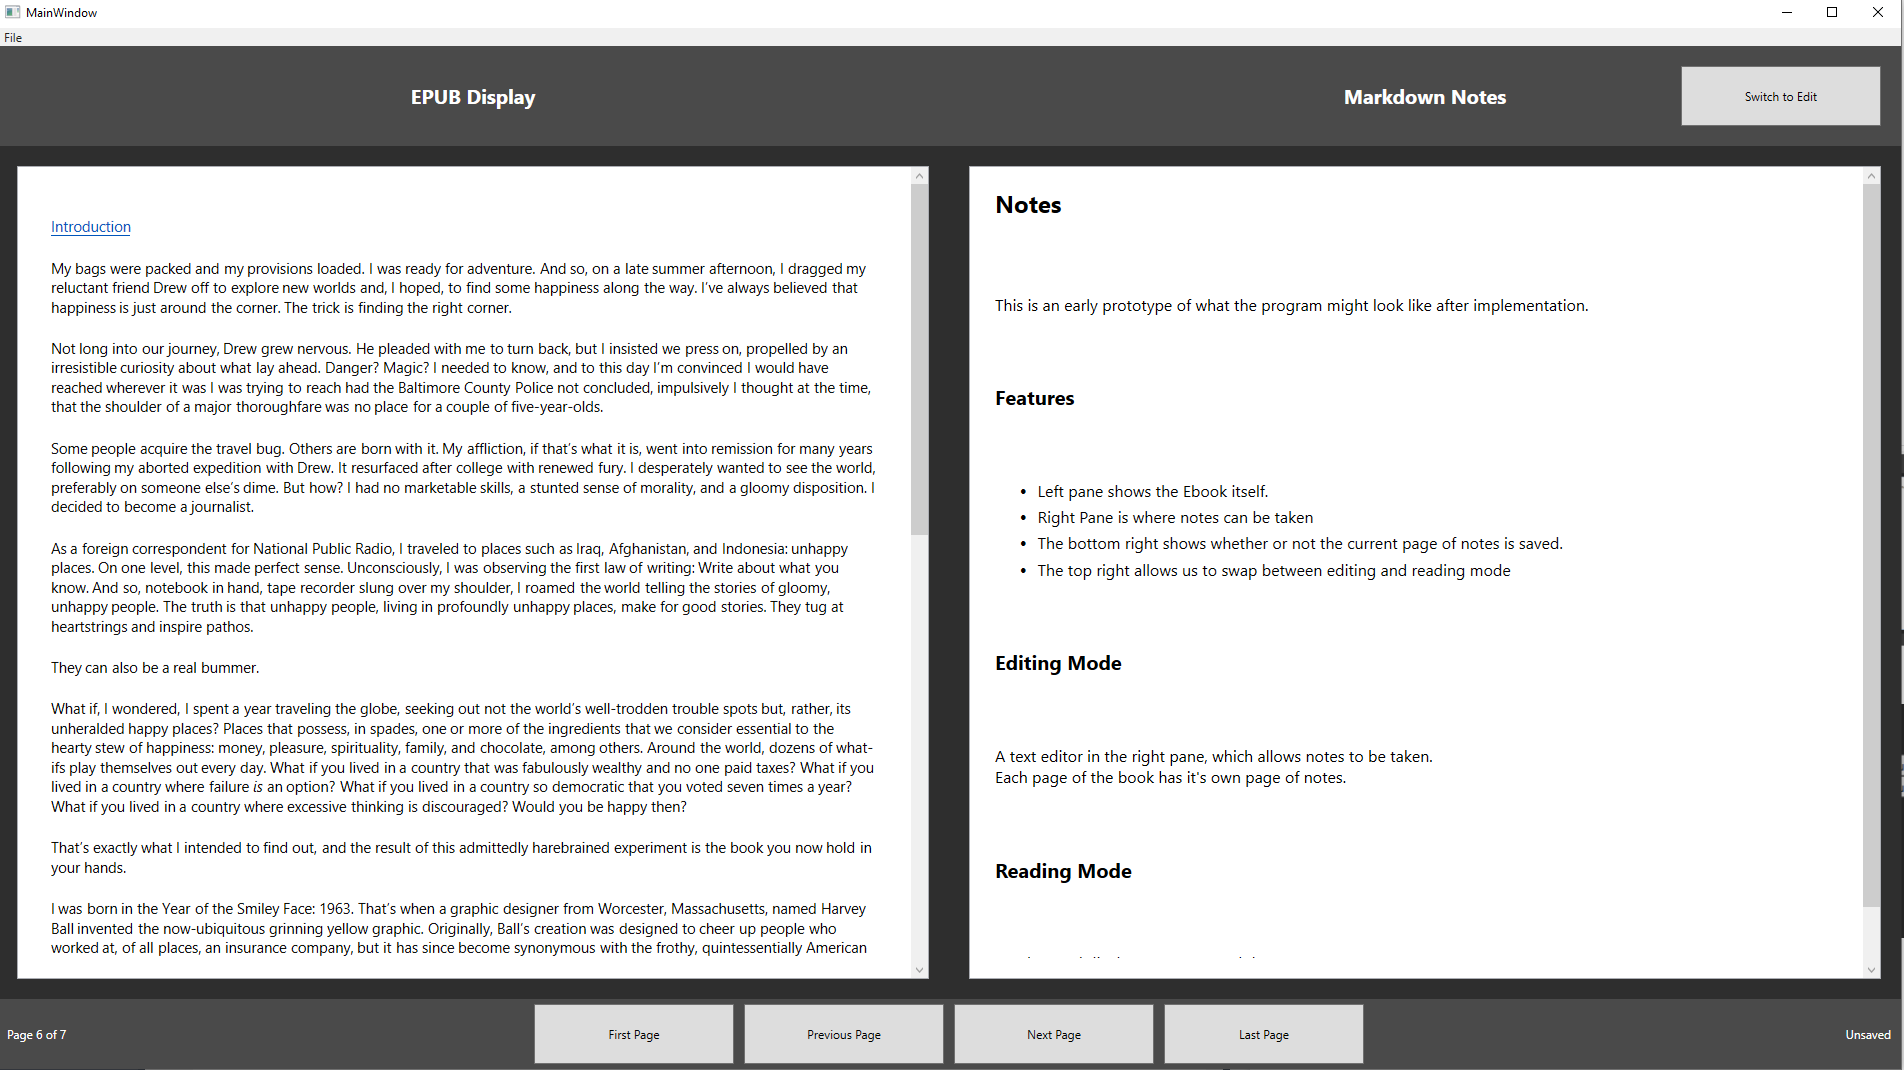
\includegraphics[width=1\textwidth]{Figures/Screenshot 2024-12-14 204334.png}}
\caption{Mock implementation of the NoteReader application, showing EPUB rendering on the left, and Note editor on the right}
\label{fig:NoteReaderMock}
\end{figure}

\begin{figure}
\centering
\subfigure[Home Page]{\label{fig:NoteReaderMock1}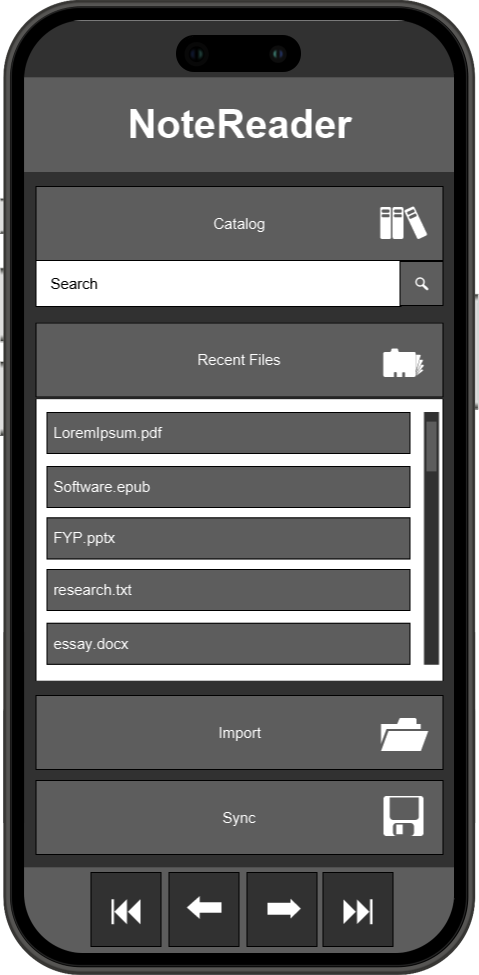
\includegraphics[width=0.35\textwidth]{Figures/home@1x.png}}
\subfigure[Document Viewing Mode]{\label{fig:NoteReaderMock1}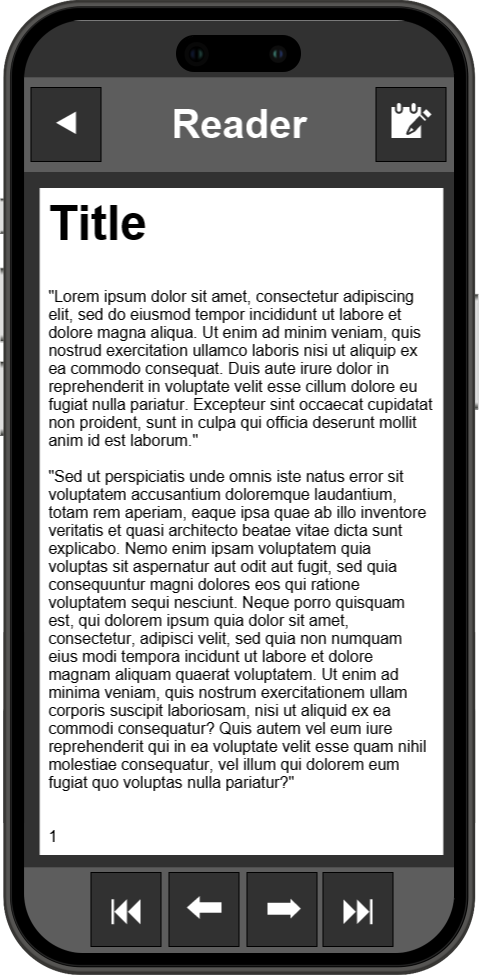
\includegraphics[width=0.35\textwidth]{Figures/Reader@1x.png}}
\subfigure[Notes Editing Mode]{\label{fig:NoteReaderMock2}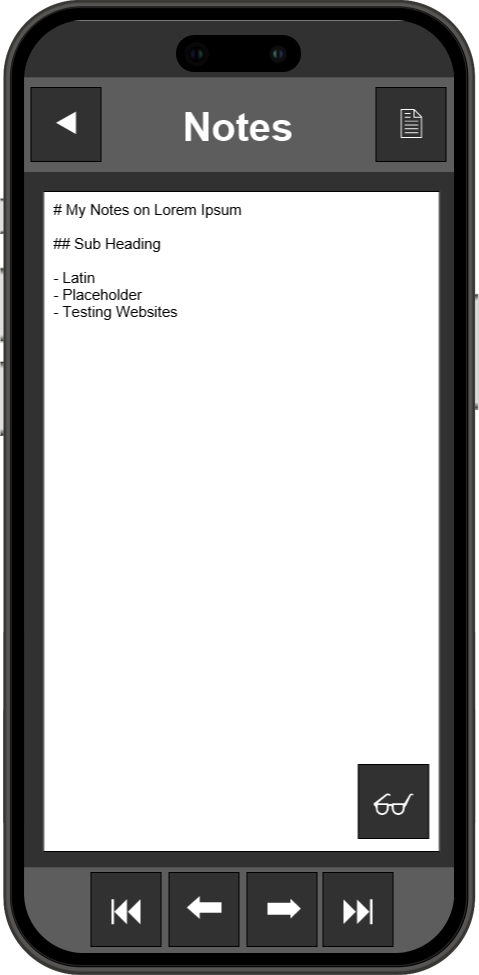
\includegraphics[width=0.35\textwidth]{Figures/Notes Editor@1x.png}}
\subfigure[Notes Rendering Mode]{\label{fig:NoteReaderMock2}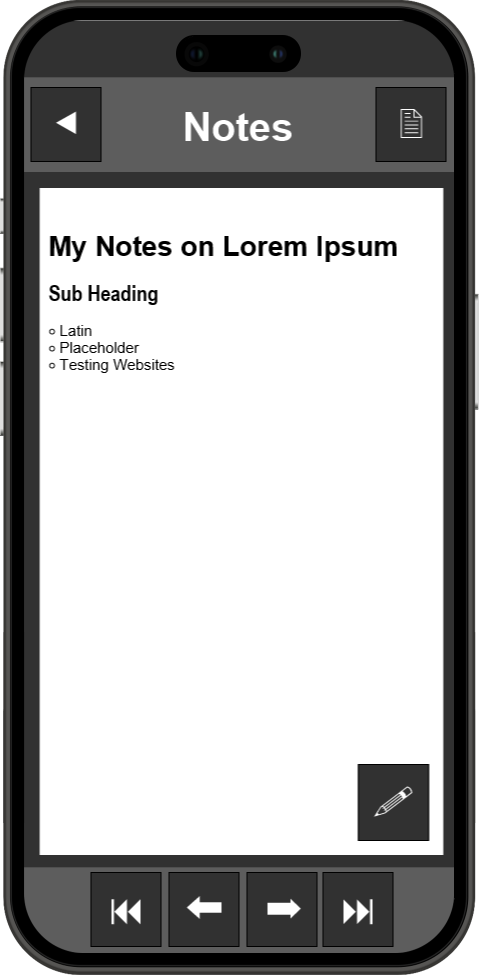
\includegraphics[width=0.35\textwidth]{Figures/Notes Render@1x.png}}
\caption{Mock implementation of the NoteReader mobile application, showing the three primary modes}
\label{fig:NoteReaderMobileMock}
\end{figure}

\begin{figure}
    \centering
    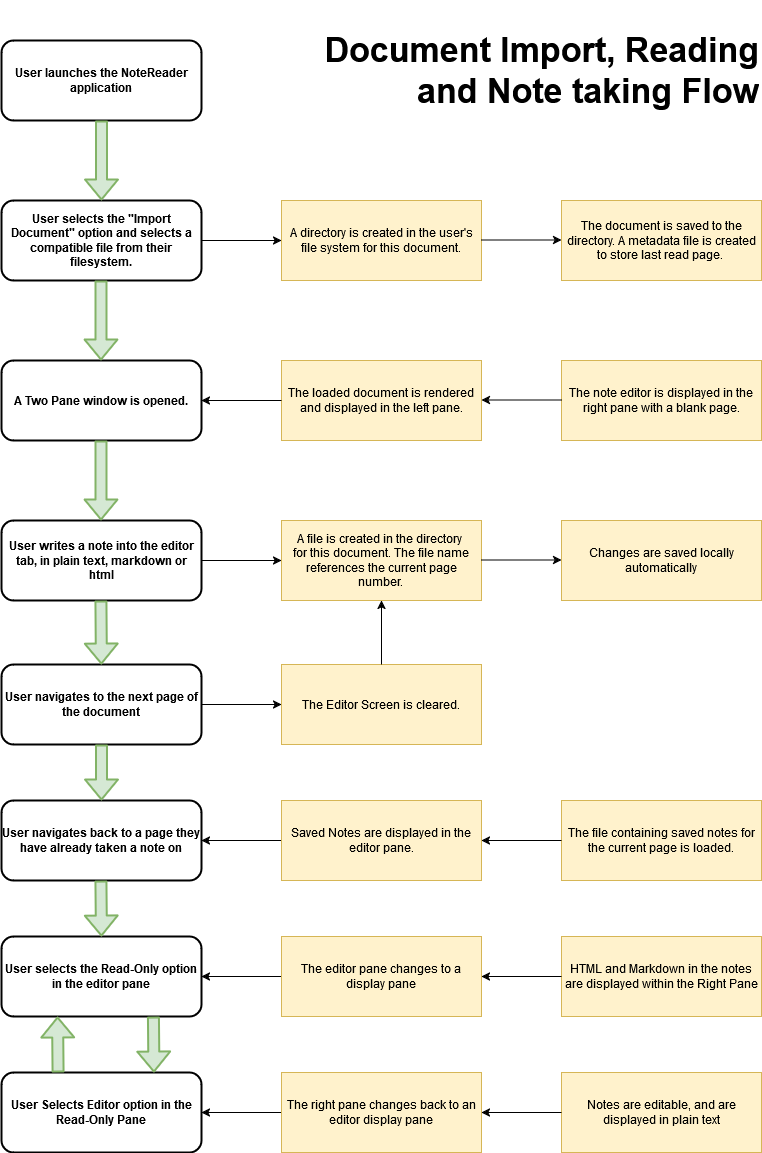
\includegraphics[width=1\linewidth]{Figures/Document_Import_Reading_NoteTaking_Flow(2).drawio.png}
    \caption{Depicting user flow from opening program, to importing documents, taking notes, and navigating between pages. }
    \label{fig:Document Import, Reading and Note taking Flow}
\end{figure}

\begin{figure}
    \centering
    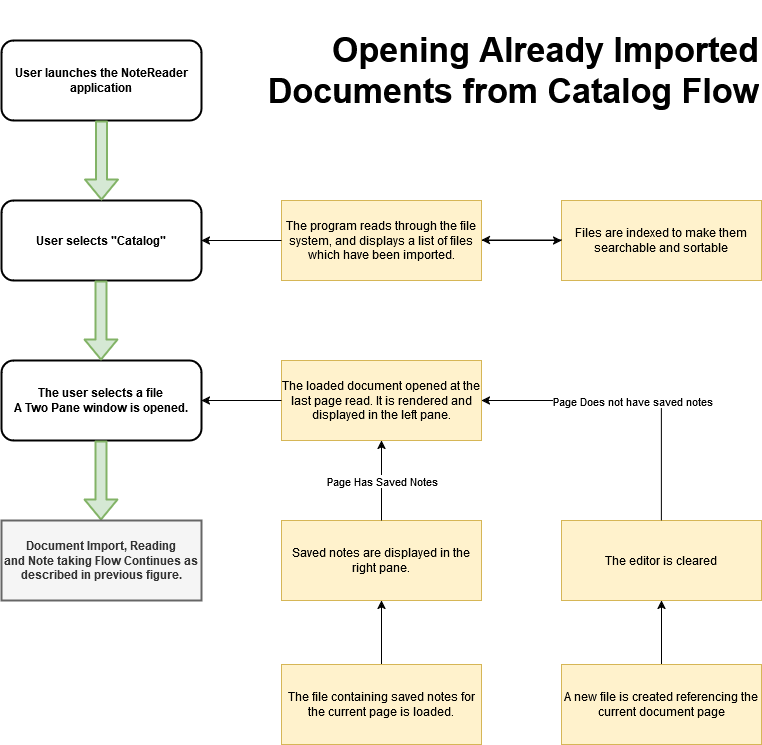
\includegraphics[width=1\linewidth]{Figures/Document_ReOpen_Reading_NoteTaking_Flow.drawio.png}
    \caption{Depicting user flow of re-opening Documents from catalogue.}
    \label{fig:OpeningAlreadyImportedDocuments}
\end{figure}

\begin{figure}
    \centering
    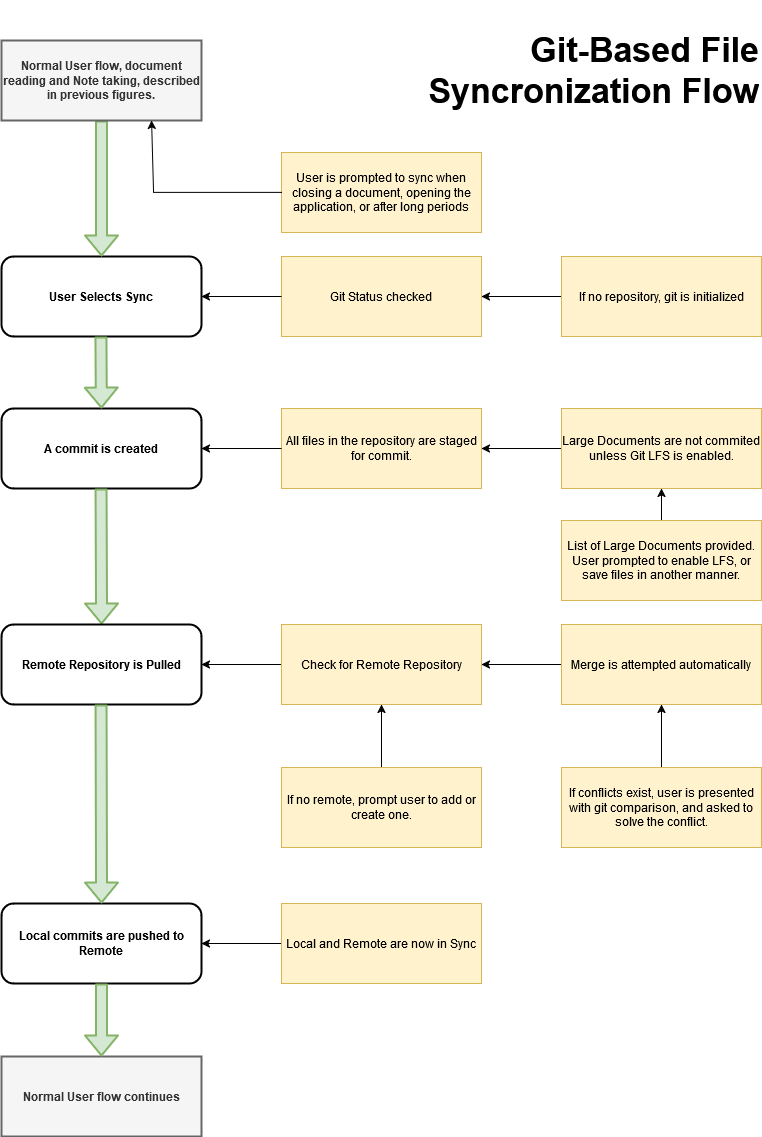
\includegraphics[width=1\linewidth]{Figures/Git_Sync_Flow.drawio.png}
    \caption{Depicting user flow of syncing files with git.}
    \label{fig:gitBasedSync}
\end{figure} % Appendix B
\chapter{Miscellaneous}

\begin{figure}
    \centering
    \includegraphics[width=1\linewidth]{Figures/Anóta(4).png}
    \caption{NoteReader Academic Poster}
    \label{fig:enter-label}
\end{figure} % Appendix C



\addtocontents{toc}{\vspace{2em}}  % Add a gap in the Contents, for aesthetics
\backmatter
\end{document}  % The End
%% ----------------------------------------------------------------
